\documentclass[a4paper]{article}
\usepackage[spanish]{babel}
\usepackage[utf8]{inputenc}
\usepackage{graphicx}
\usepackage{biblatex}
\usepackage{enumerate}
\usepackage{csquotes}
\usepackage{braket}
\usepackage{amsmath}

\title{Spiking neurons}
\begin{document}
\maketitle
\section{Estabilidad}
Las ecuaciones que describen al sistema son:
$$\dot{r}=\frac{\Delta}{\pi}+2rv$$
$$\dot{v}=v^2+\bar{\eta}+Jr-\pi^2 r^2 + I(t)$$
Para saber las nulclinas tomamos $\dot{r}=0$ y $\dot{v} = 0$.
$$\frac{\Delta}{\pi}+2rv=0 \Rightarrow r = -\frac{\Delta}{2 \pi v}$$
$$v^2+\bar{\eta}+Jr-\pi^2 r^2 + I(t) = 0$$
Los puntos de estabilidad los obtenemos con los puntos de corte de estas dos funciones.
El campo vectorial lo obtenemos dando valores a r y a v en el el sistema:
$$\dot{r}=\frac{\Delta}{\pi}+2rv$$
$$\dot{v}=v^2+\bar{\eta}+Jr-\pi^2 r^2 + I(t)$$
siendo $\dot{r}$ la componente en x de cada vector y $\dot{v}$ la componente en y. 
Para saber el tipo de estabilidad en cada punto tomamos las funciones:
$$f(r,v) = \frac{\Delta}{\pi}+2rv$$
$$g(r,v) = v^2+\bar{\eta}+Jr-\pi^2 r^2 + I(t)$$
$$
\begin{pmatrix} \dot{r} \\ \dot{v} \end{pmatrix} = 
\begin{pmatrix}
\frac{\partial f}{\partial r} & \frac{\partial f}{\partial v} \\
\frac{\partial g}{\partial r} & \frac{\partial g}{\partial v}
\end{pmatrix}
\begin{pmatrix} r \\ v \end{pmatrix}
$$
$$
\begin{pmatrix} \dot{r} \\ \dot{v} \end{pmatrix} = 
\begin{pmatrix}
2v & 2r \\
J - 2\pi^2 r & 2v
\end{pmatrix}
\begin{pmatrix} r \\ v \end{pmatrix}
$$
$$Tr = 4v$$
$$det = 4v^2 - 2rJ + 4\pi^2 r^2$$
\section{Pasos a seguir}
día 12/02/2020 \\
El programa funciona igual que en el paper. (PONER ALGUNAS IMÁGENES). El próximo paso a seguir es comprobar el diagrama de fases.\\

día 13/02/2020\\
Sabemos que $r = nºspiking Neurons/(N*dt)$\\
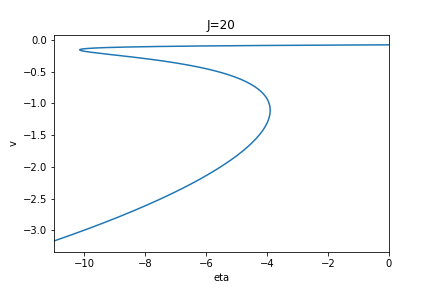
\includegraphics[scale=0.7]{v_vs_eta_J20.png}\\
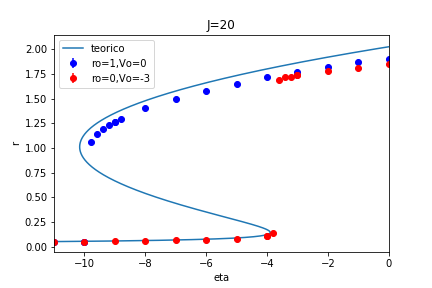
\includegraphics[scale=0.7]{r_vs_eta_J20.png}\\
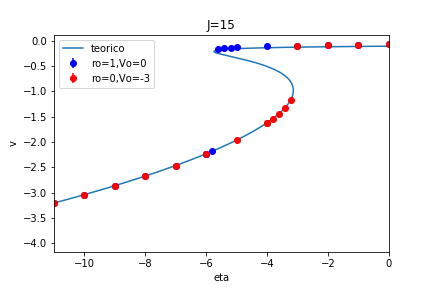
\includegraphics[scale=0.7]{v_vs_eta_J15.png}\\
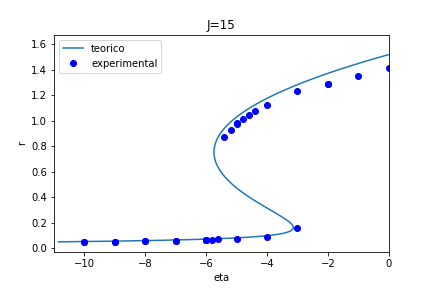
\includegraphics[scale=0.7]{r_vs_eta_J15.png}\\
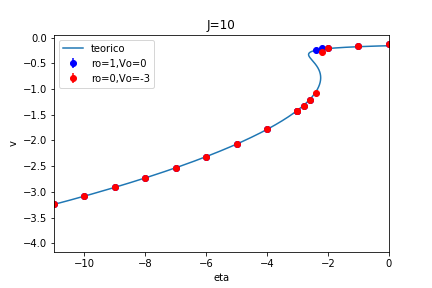
\includegraphics[scale=0.7]{v_vs_eta_J10.png}\\
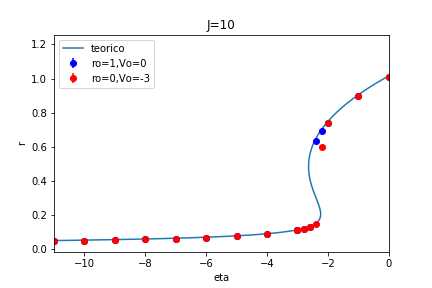
\includegraphics[scale=0.7]{r_vs_eta_J10.png}\\
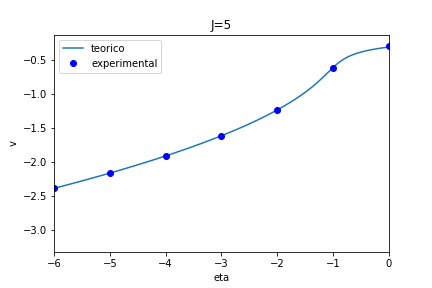
\includegraphics[scale=0.7]{v_vs_eta_J5.png}\\
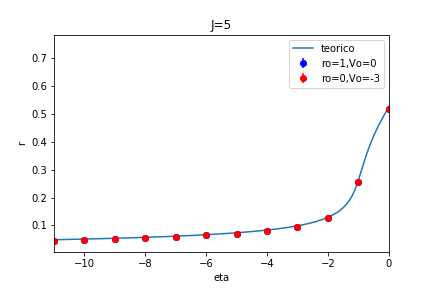
\includegraphics[scale=0.7]{r_vs_eta_J5.png}\\
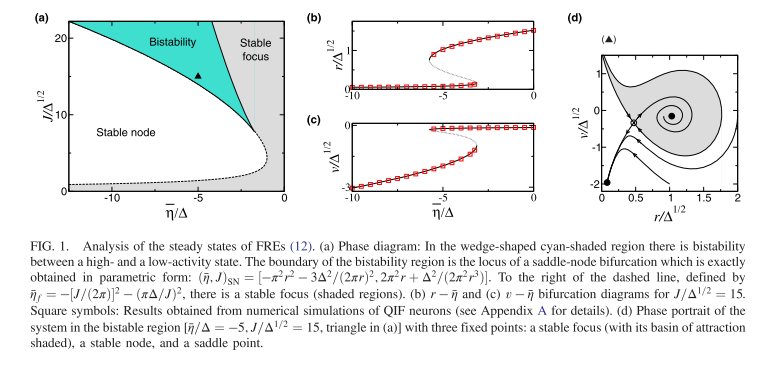
\includegraphics[scale=0.4]{diagramaspaper.png}\\

En el caso práctico dejamos el programa correr por 15 unidades temporales con las condiciones iniciales. Luego quitamos esas condiciones y dejamos correr el programa por 60 unidades temporales más, tomando la media de las últimas 30 unidades temporales.\\
Además tomamos el error de la media como $1.96\cdot SE$. Cuya fórmula es:
$$SE = \frac{\sigma}{\sqrt{M}}$$
con
$$\sigma = \sqrt{\frac{1}{M}\left(\sum^M_ {i=1} (x^2_i)-M\mu^2\right)} $$
Para demostrar la biestabilidad primero vamos a la zona de estabilidad más activa para $ J = 15$:
$r\simeq 1$ y $ v\simeq 0$
para obtener  $r = 1$
$$nºspikingNeurons/Ndt = 1$$
con $N = 10^4$ y $dt = 10^{-4}$
entonces en cada intervalo temporal
$$nºspikingNeurons = 1$$
Esto lo mantenemos durante 15s y luego dejamos 30s al sistema para relajarse.
Ahora nos vamos a la zona estable de bajo firing:
$r\simeq 0$ y $ v\simeq -3$\\

Hacemos lo mismo con $J = 20$\\
Zona bajo firing:\\
$r\simeq 0$ y $ v\simeq -3$\\
Zona alto firing:\\
$r\simeq 1$ y $ v\simeq 0$\\

día 18/02/2020\\
Ahora establecemos conexiones aleatorias según el modelo de Erdos-Renyi.\\
Para una conectividad = 10 tenemos:\\
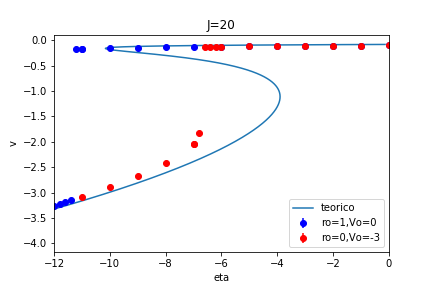
\includegraphics[scale=0.7]{v_vs_eta_J20_con10_2.png}\\
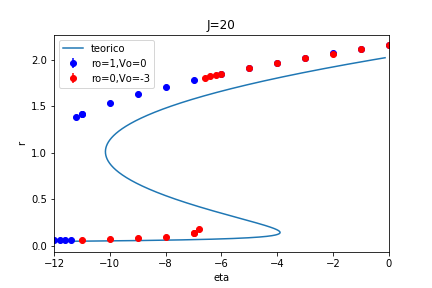
\includegraphics[scale=0.7]{r_vs_eta_J20_con10_2.png}\\
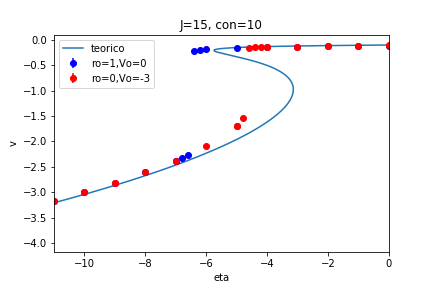
\includegraphics[scale=0.7]{v_vs_eta_J15_con10_2.png}\\
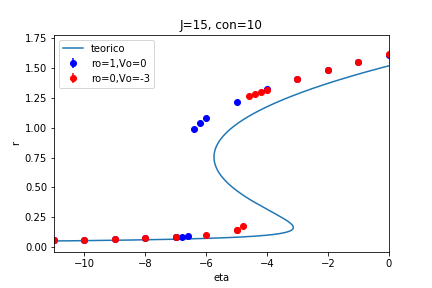
\includegraphics[scale=0.7]{r_vs_eta_J15_con10_2.png}\\
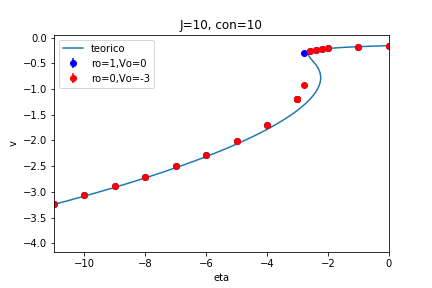
\includegraphics[scale=0.7]{v_vs_eta_J10_con10_2.png}\\
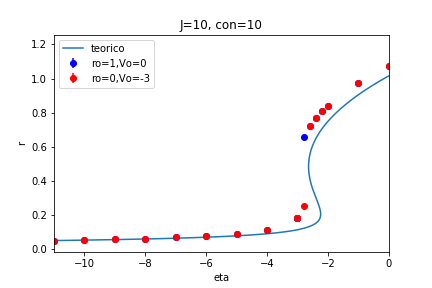
\includegraphics[scale=0.7]{r_vs_eta_J10_con10_2.png}\\
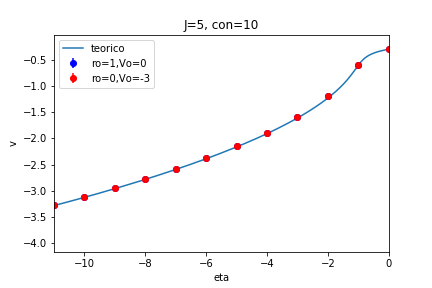
\includegraphics[scale=0.7]{v_vs_eta_J5_con10_2.png}\\
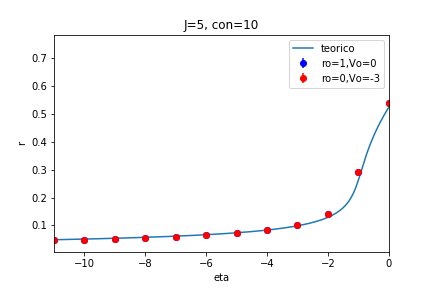
\includegraphics[scale=0.7]{r_vs_eta_J5_con10_2.png}\\

\section{redes modulares}
Tomamos una red de 10000 neuronas y la separamos en 4 módulos de 2500 neuronas cada uno. Tomamos una conectividad 10 para cada módulo. Para que esto pase, la probabilidad de conexión debe ser  $p=4$.\\
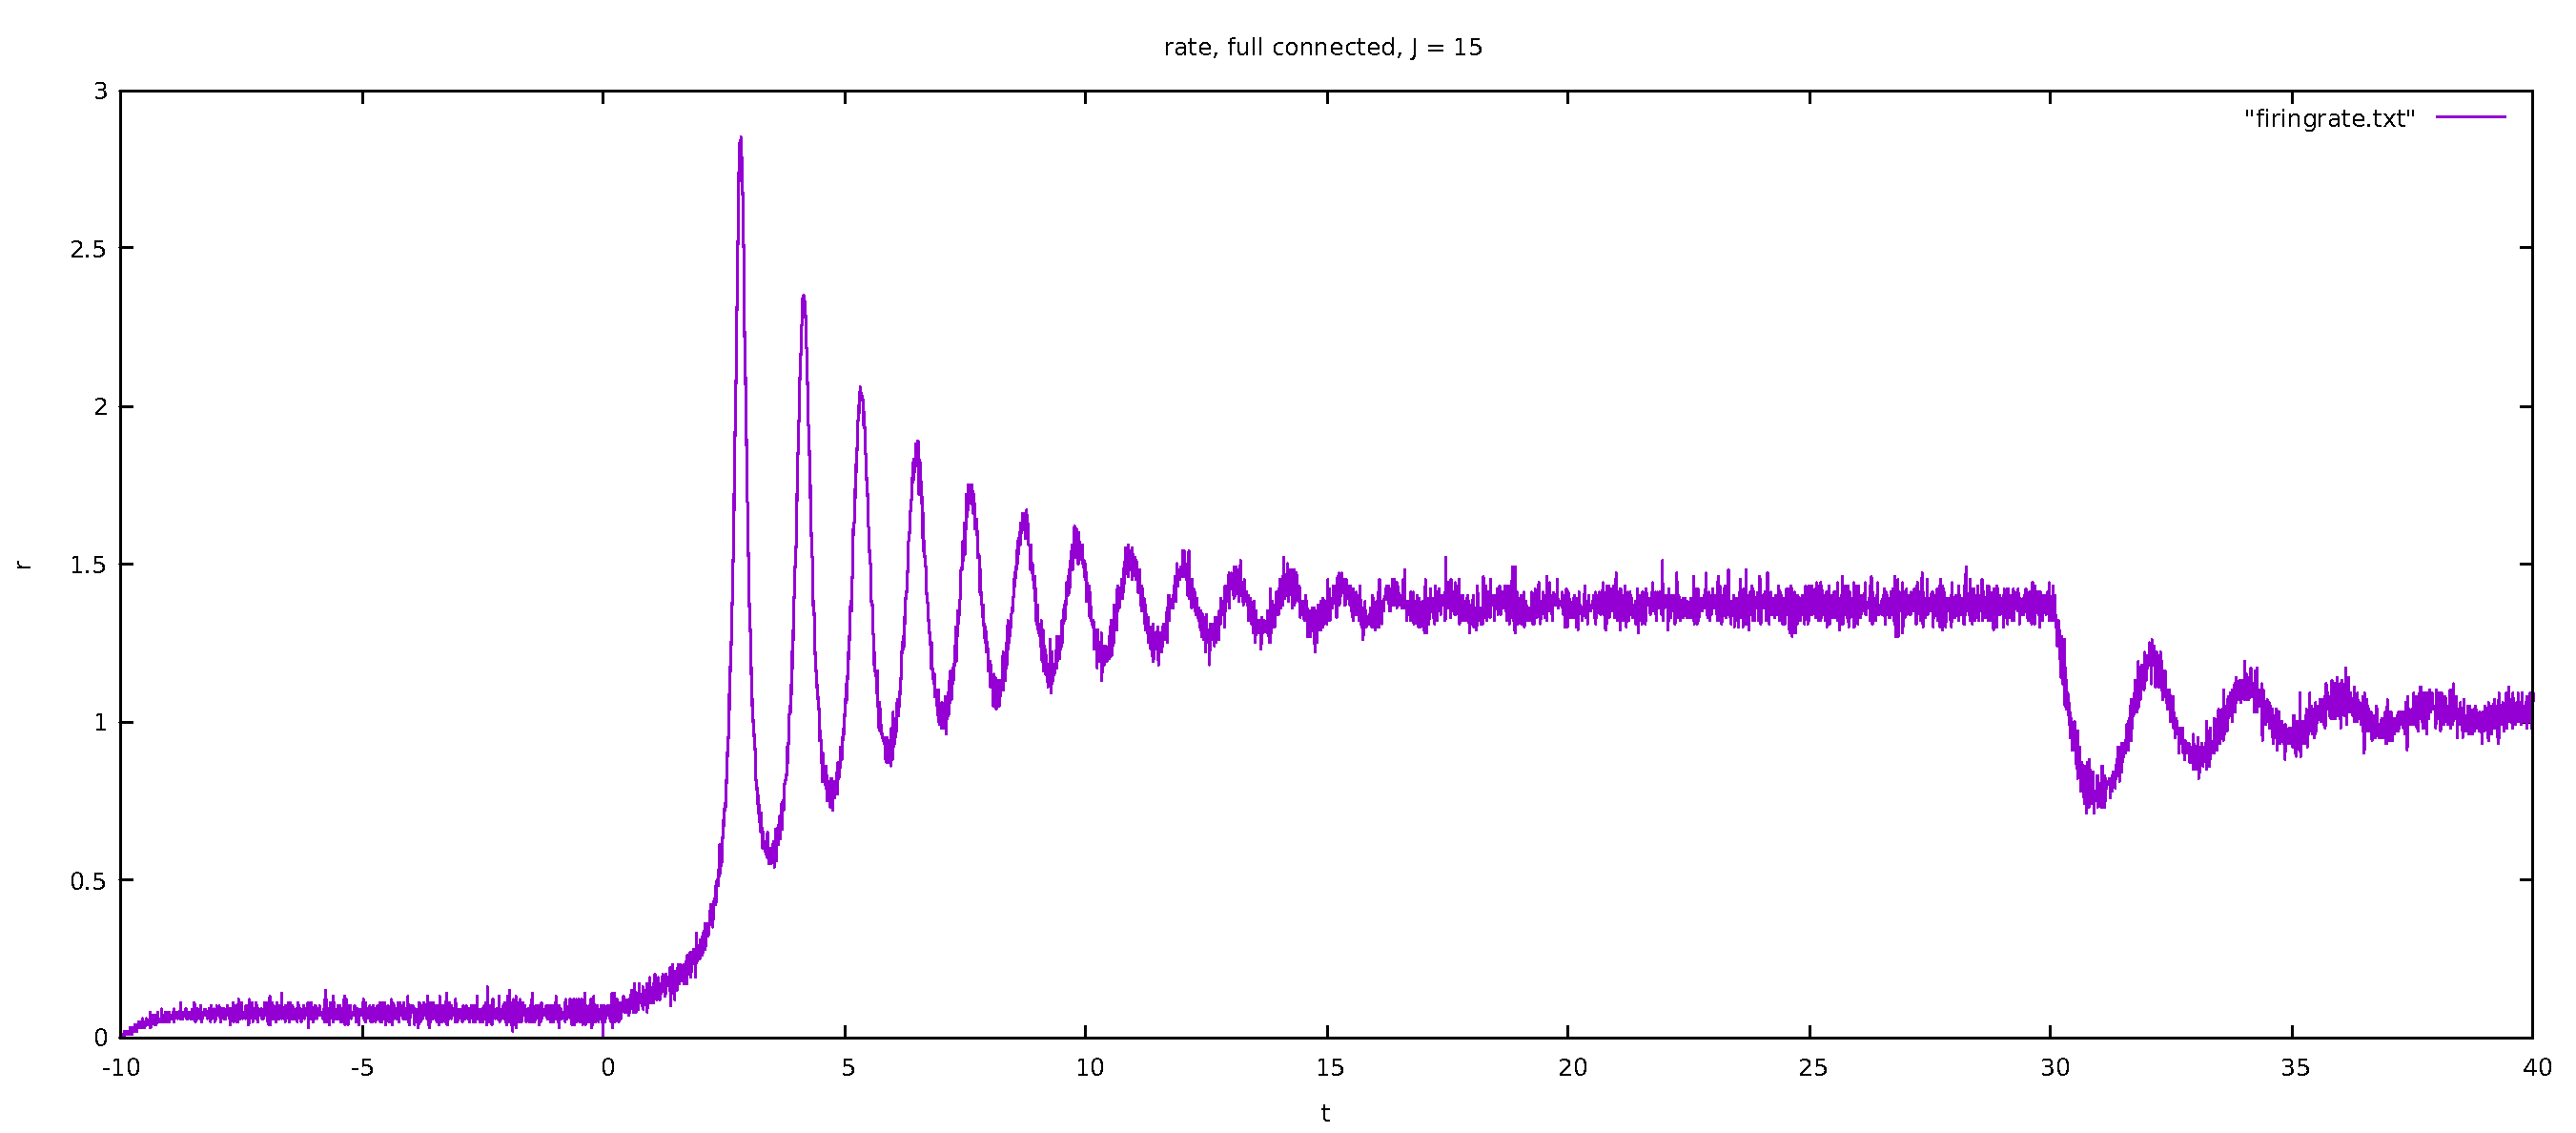
\includegraphics[scale=0.2]{fullconnected_rate_J15.pdf}\\
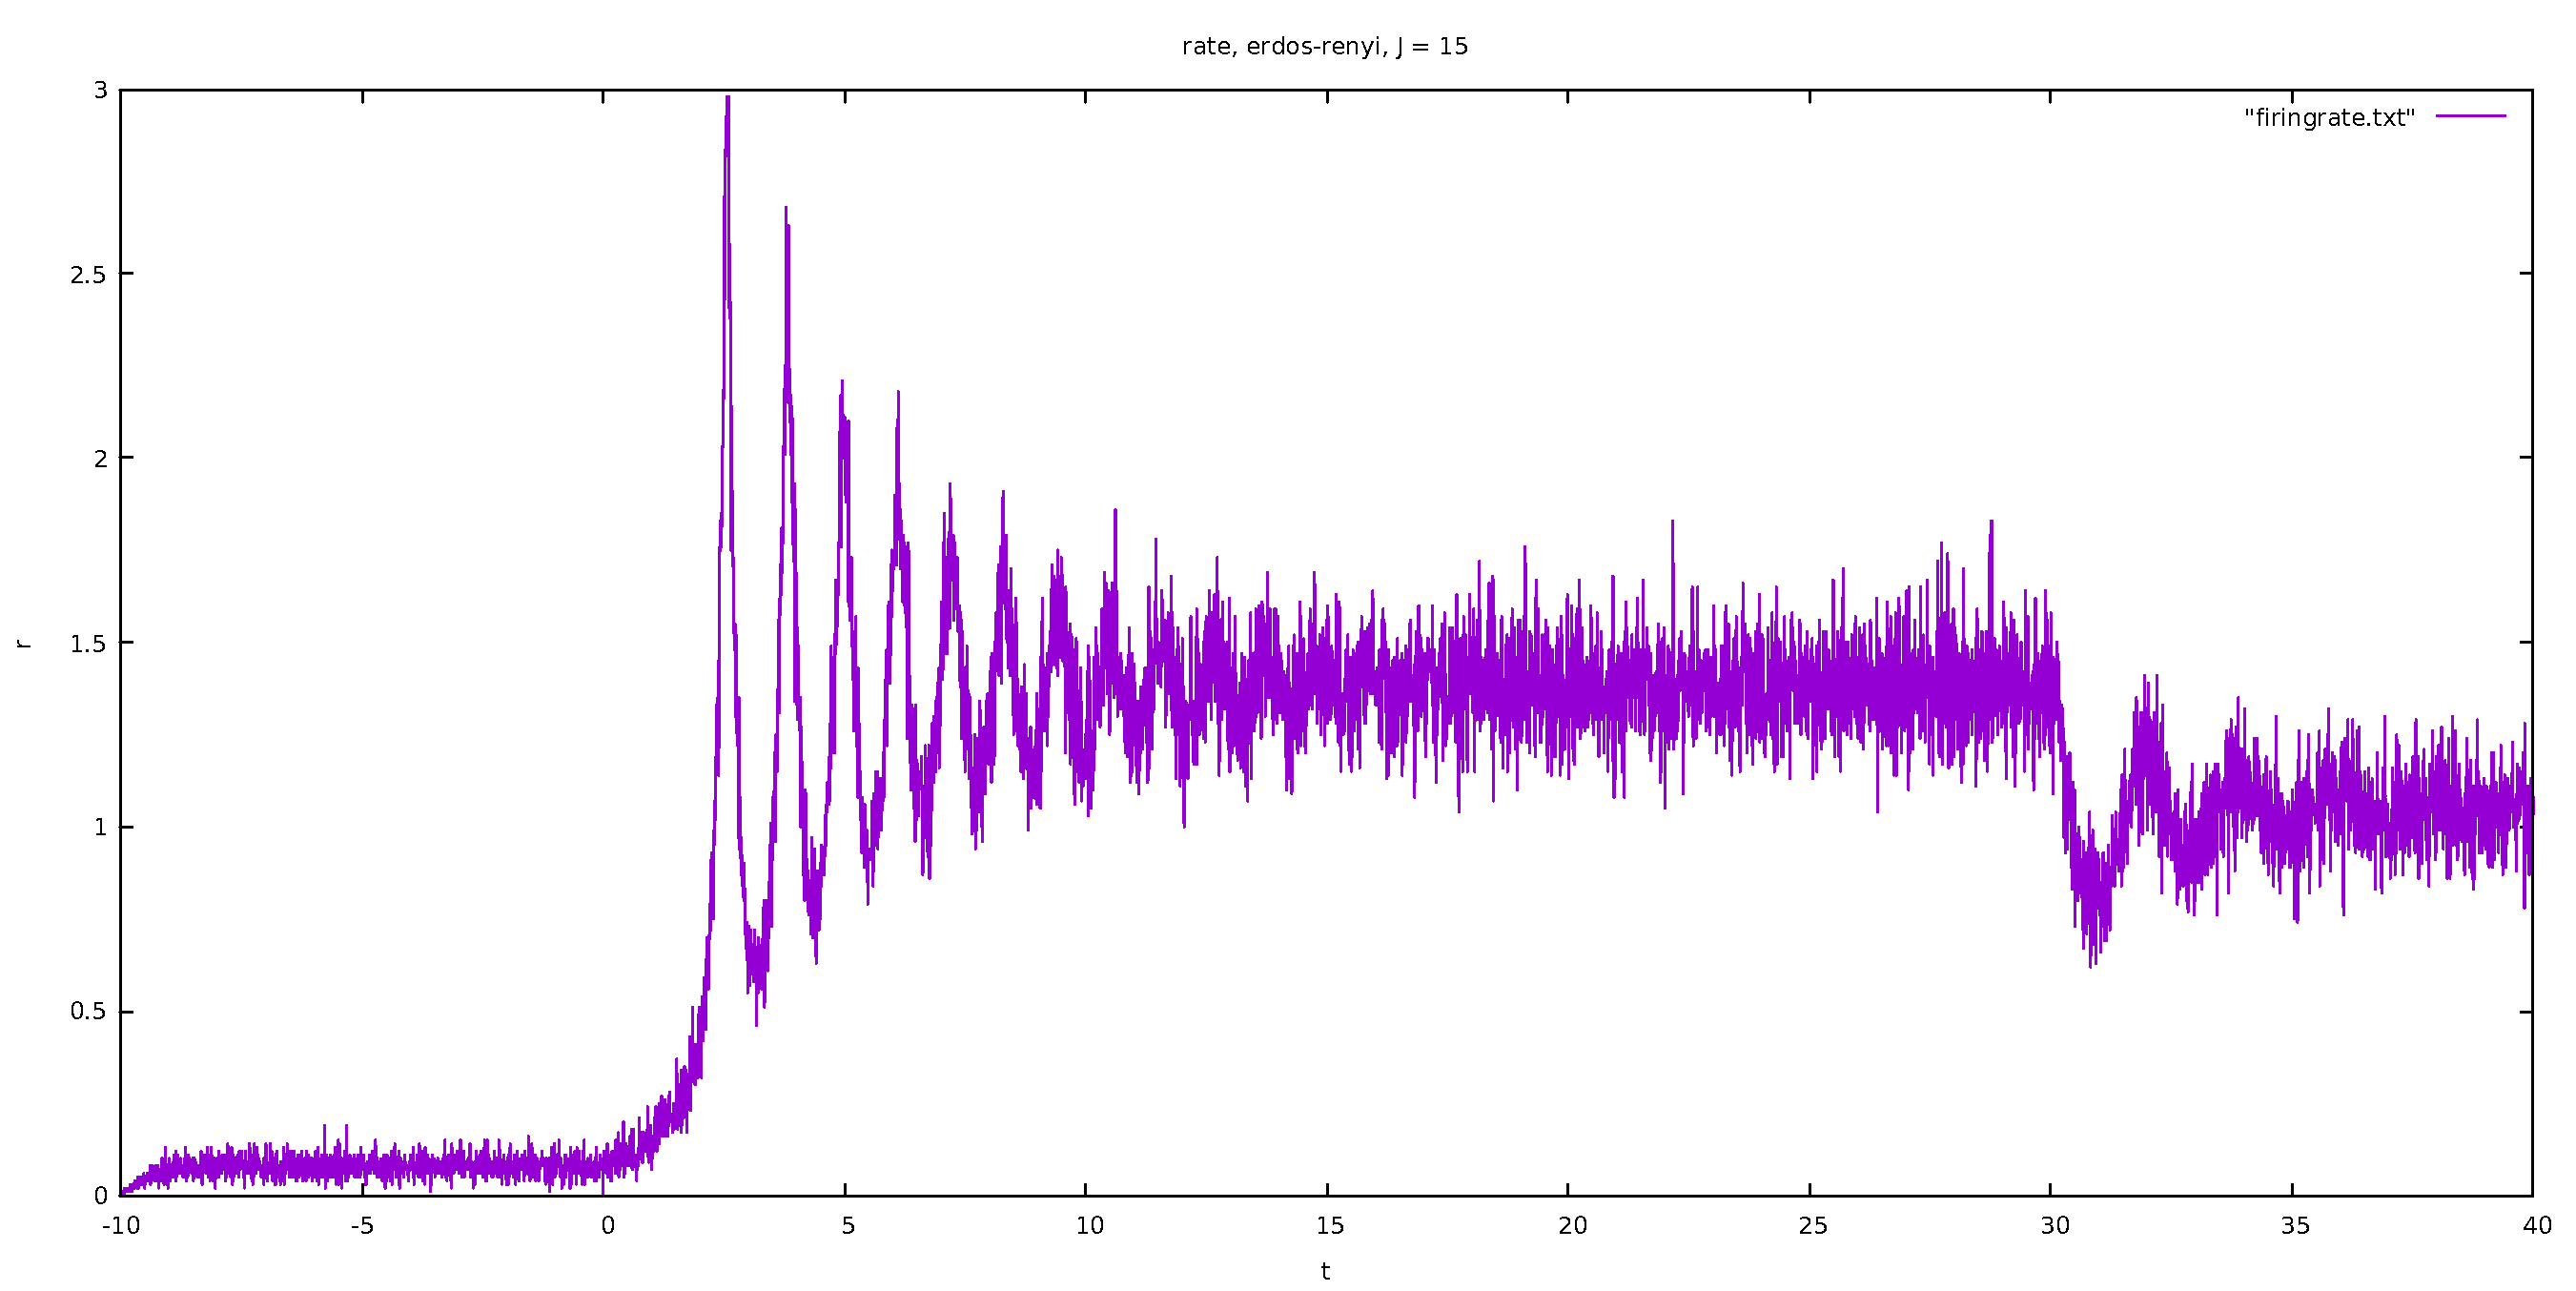
\includegraphics[scale=0.2]{erdos_rate_J15.pdf}\\
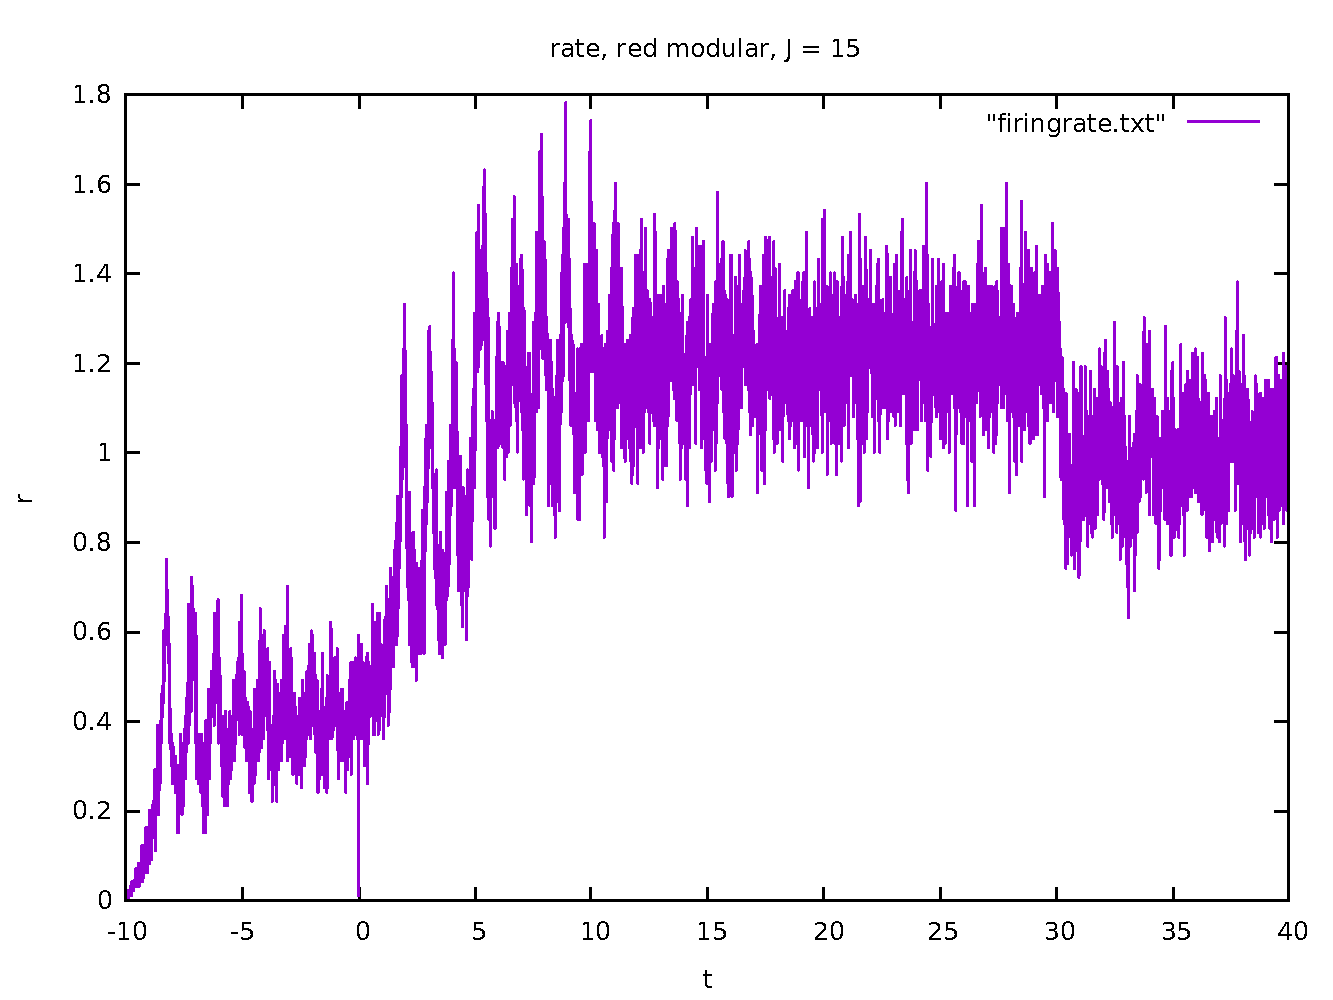
\includegraphics[scale=0.4]{modular_rate_J15.pdf}\\
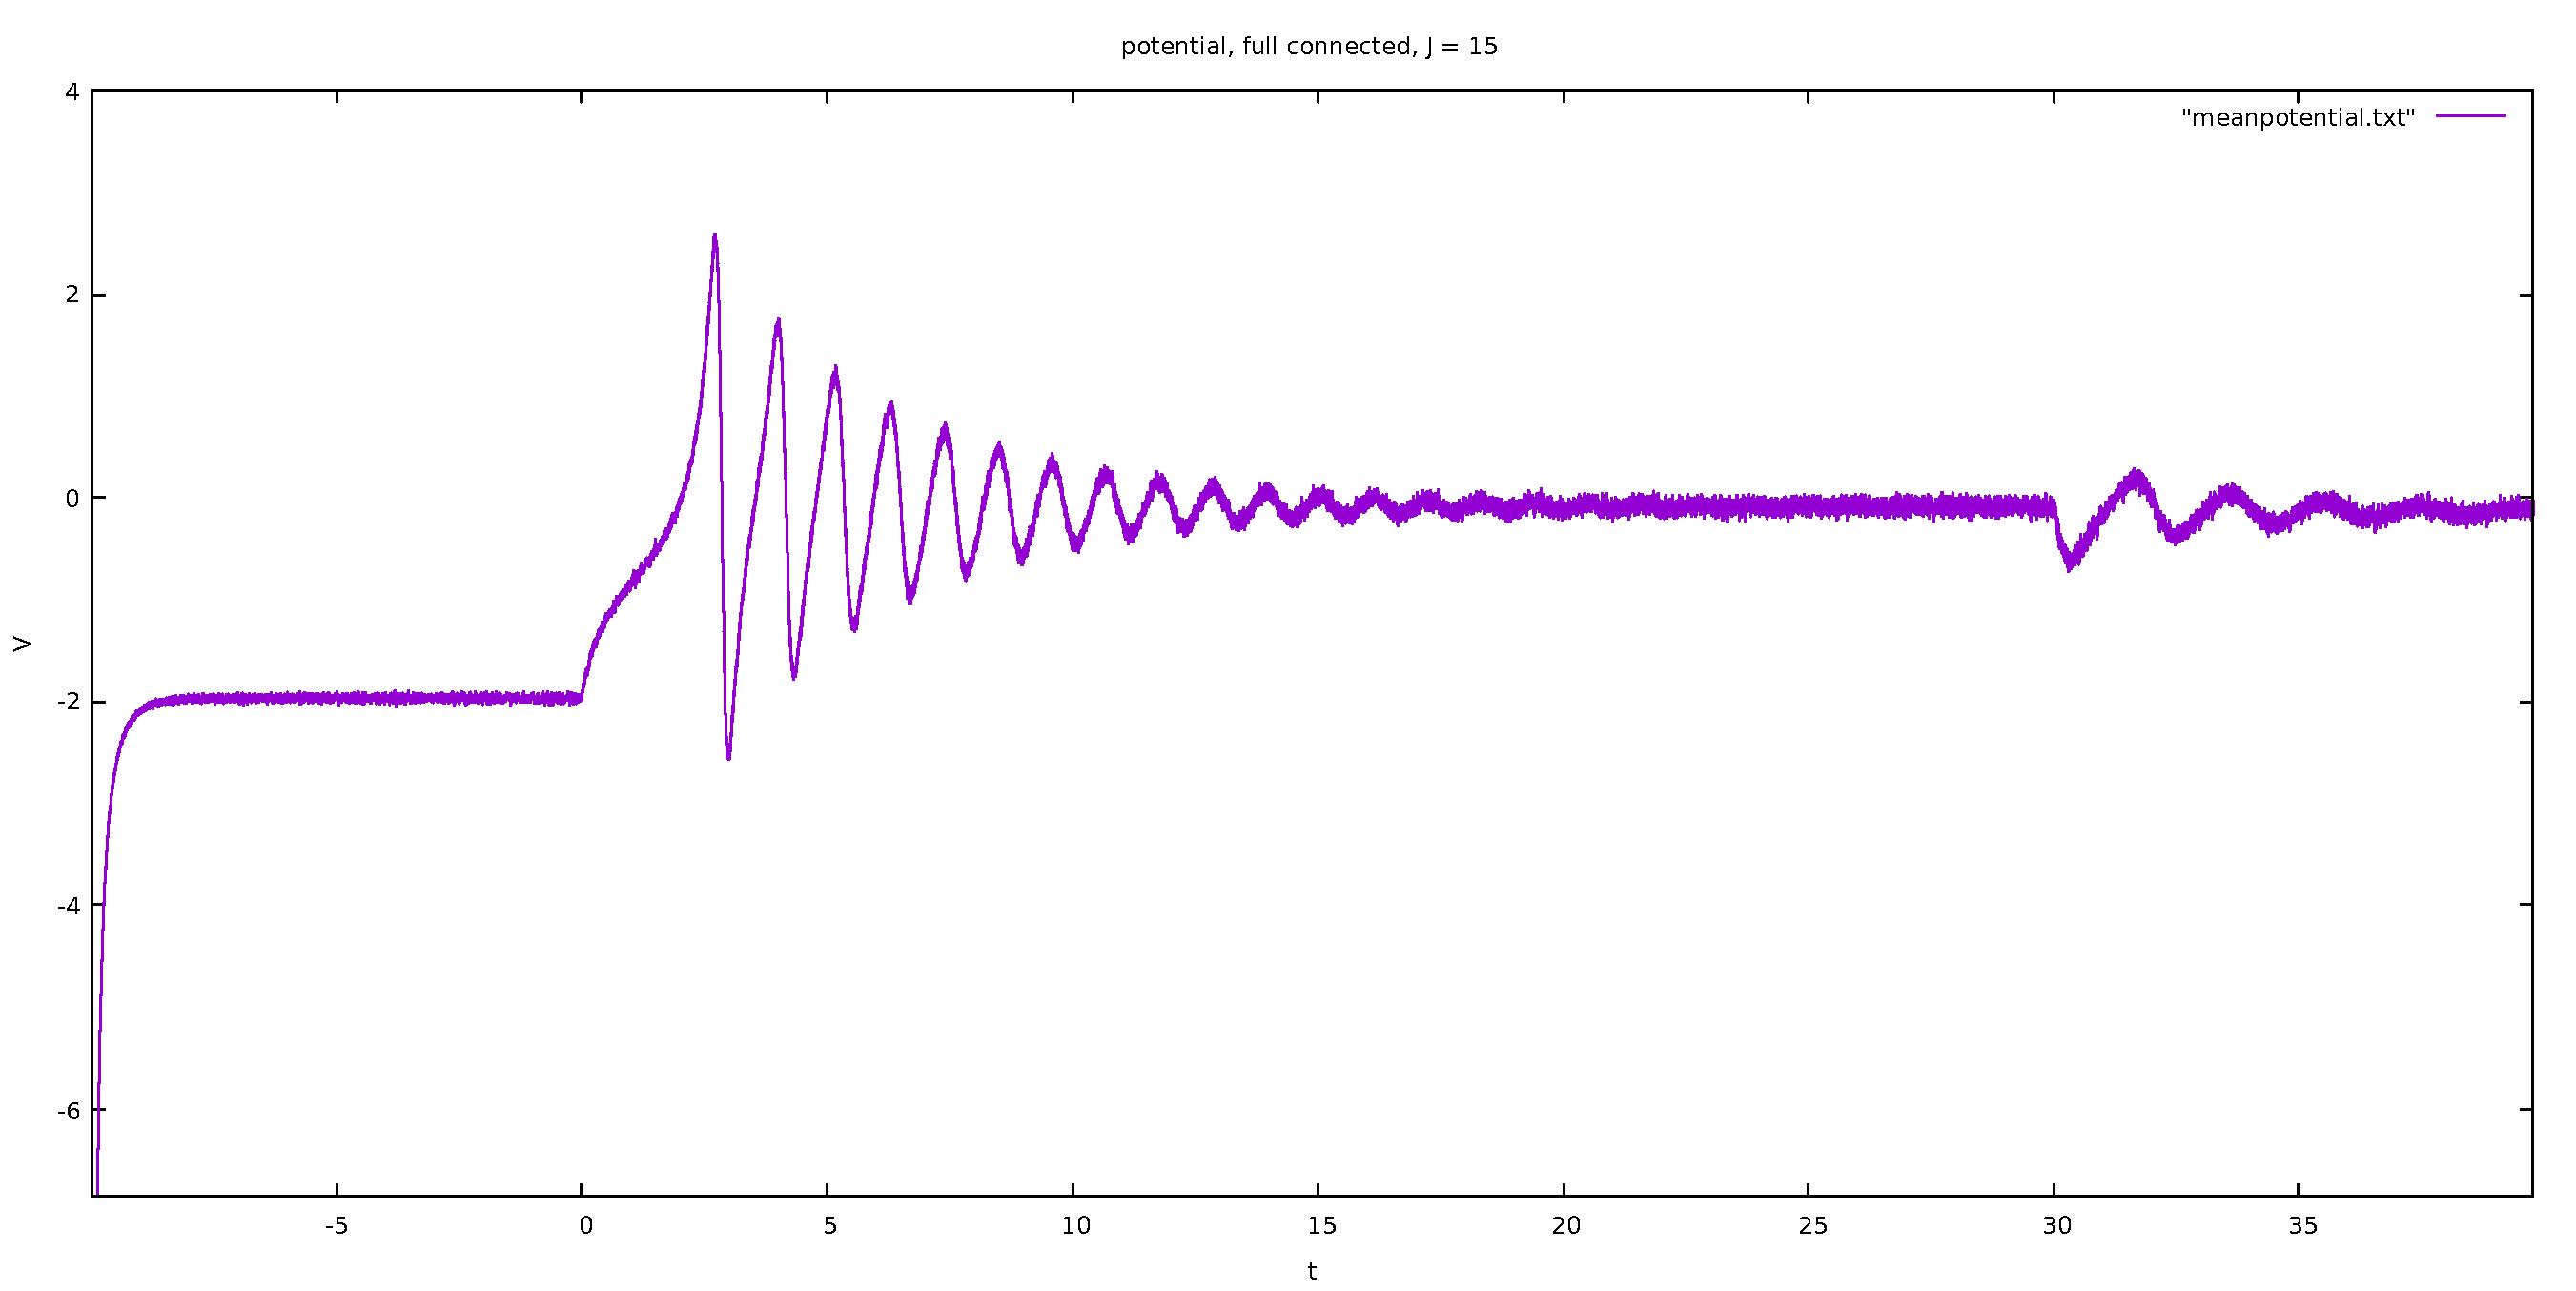
\includegraphics[scale=0.2]{fullconnected_pot_J15.pdf}\\
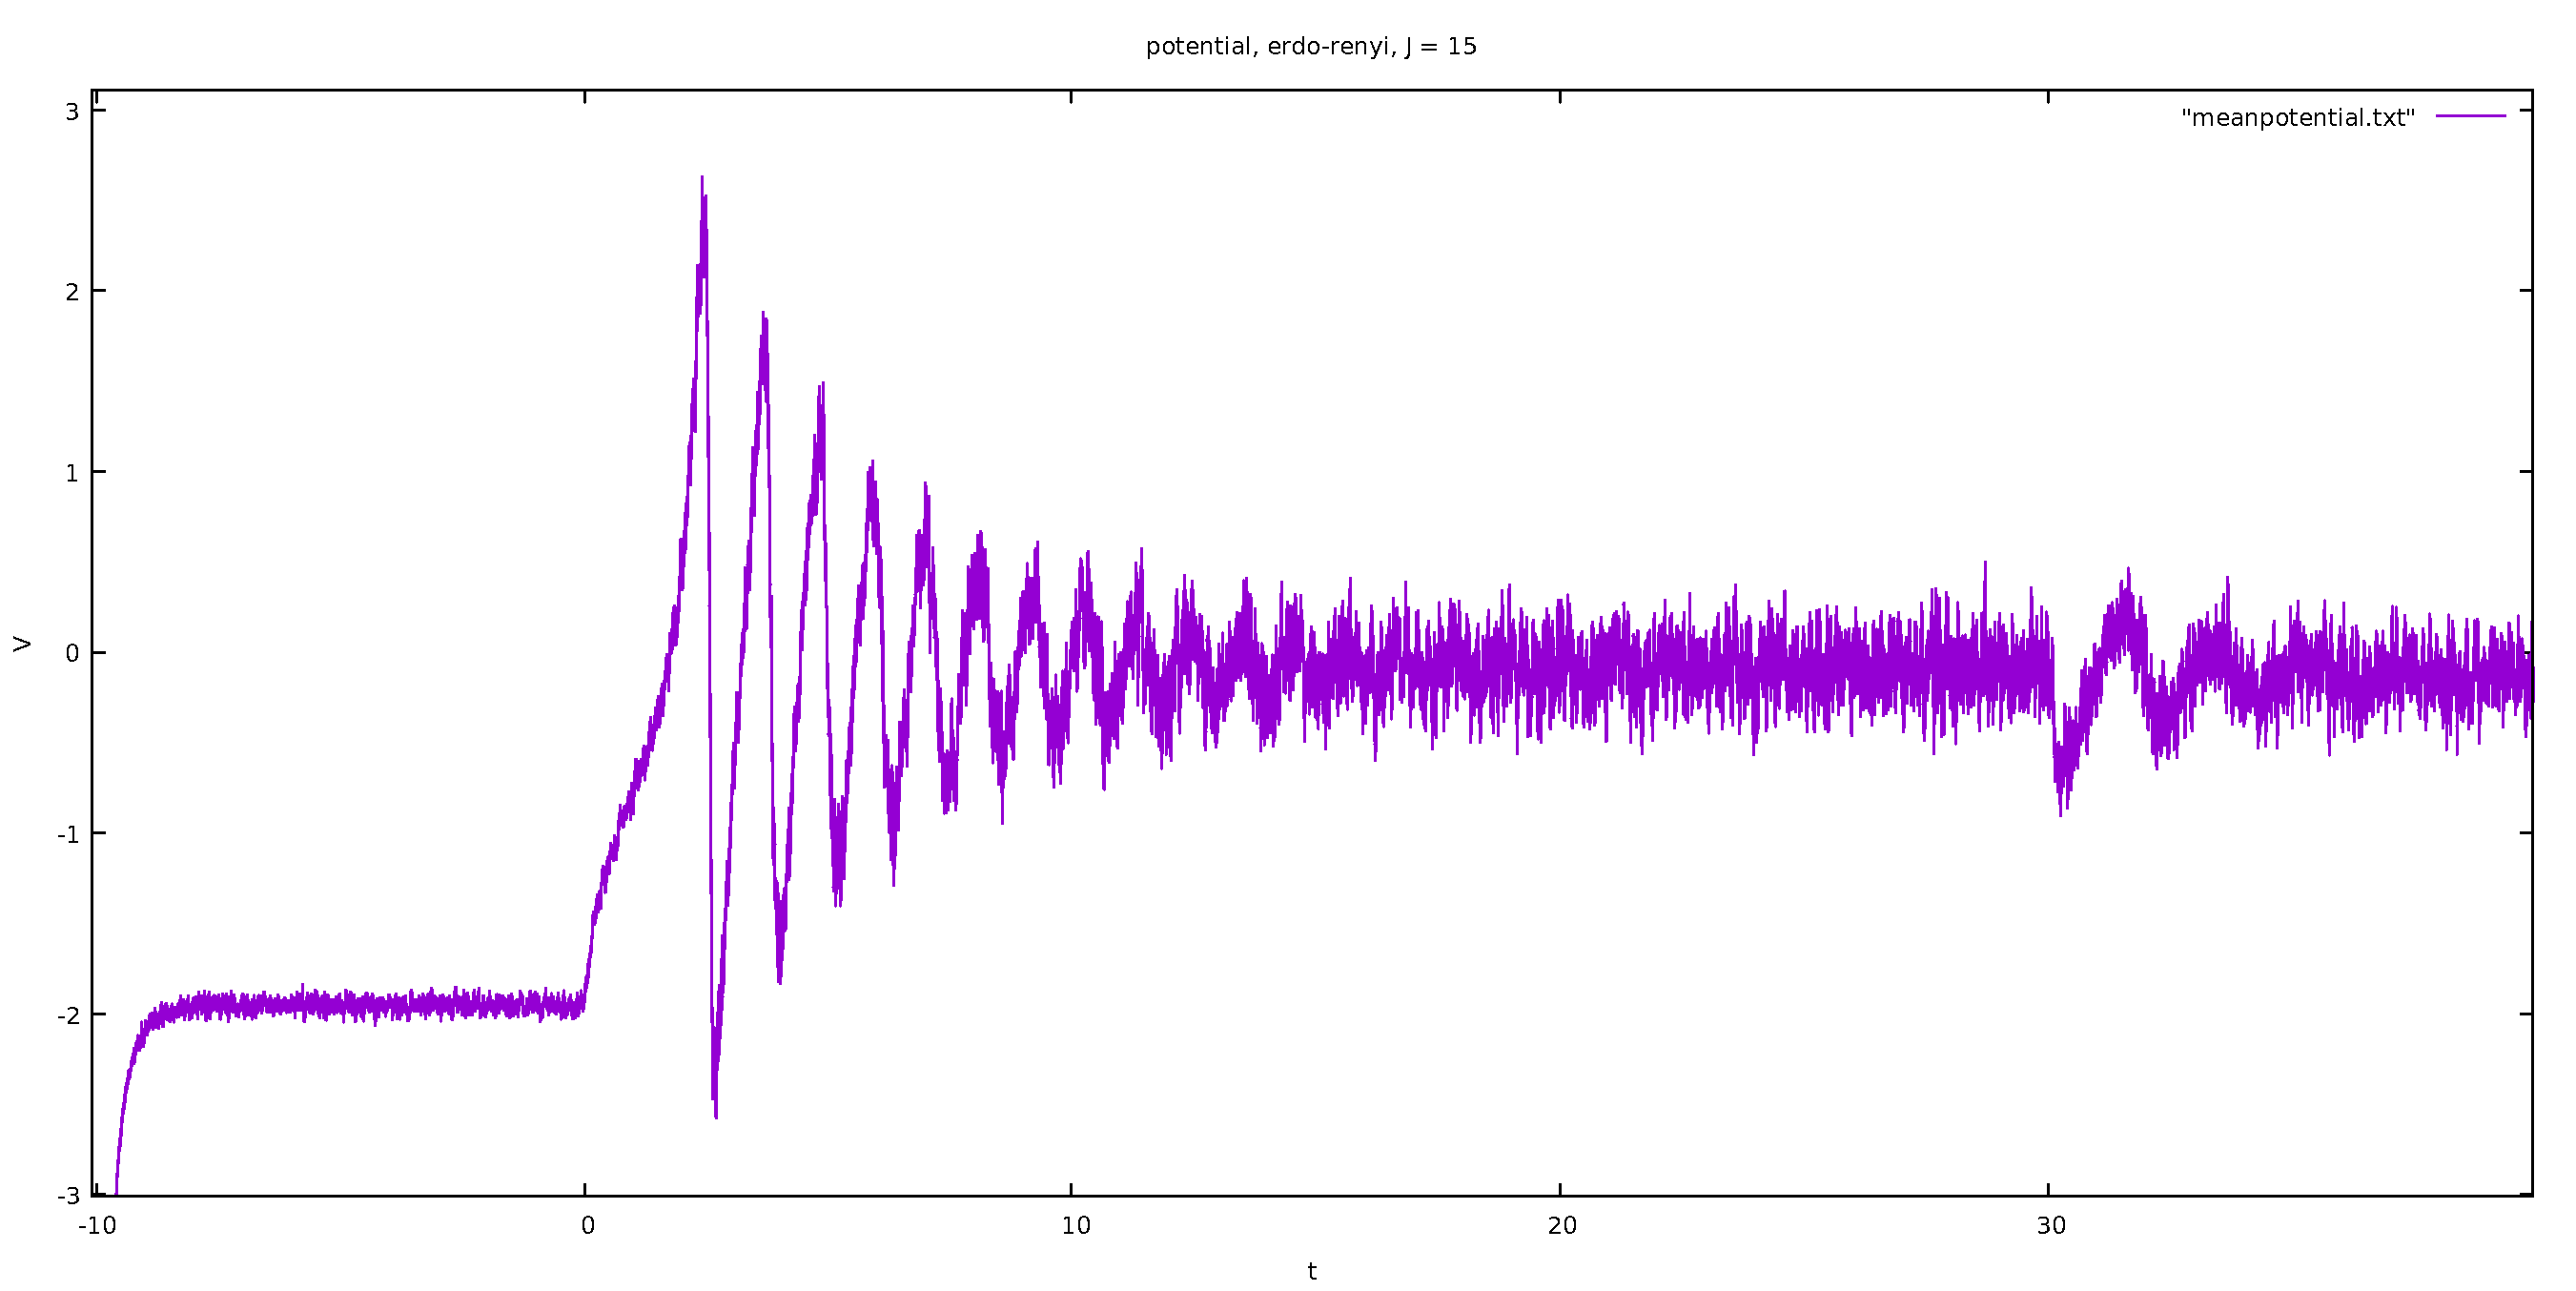
\includegraphics[scale=0.2]{erdos_pot_J15.pdf}\\
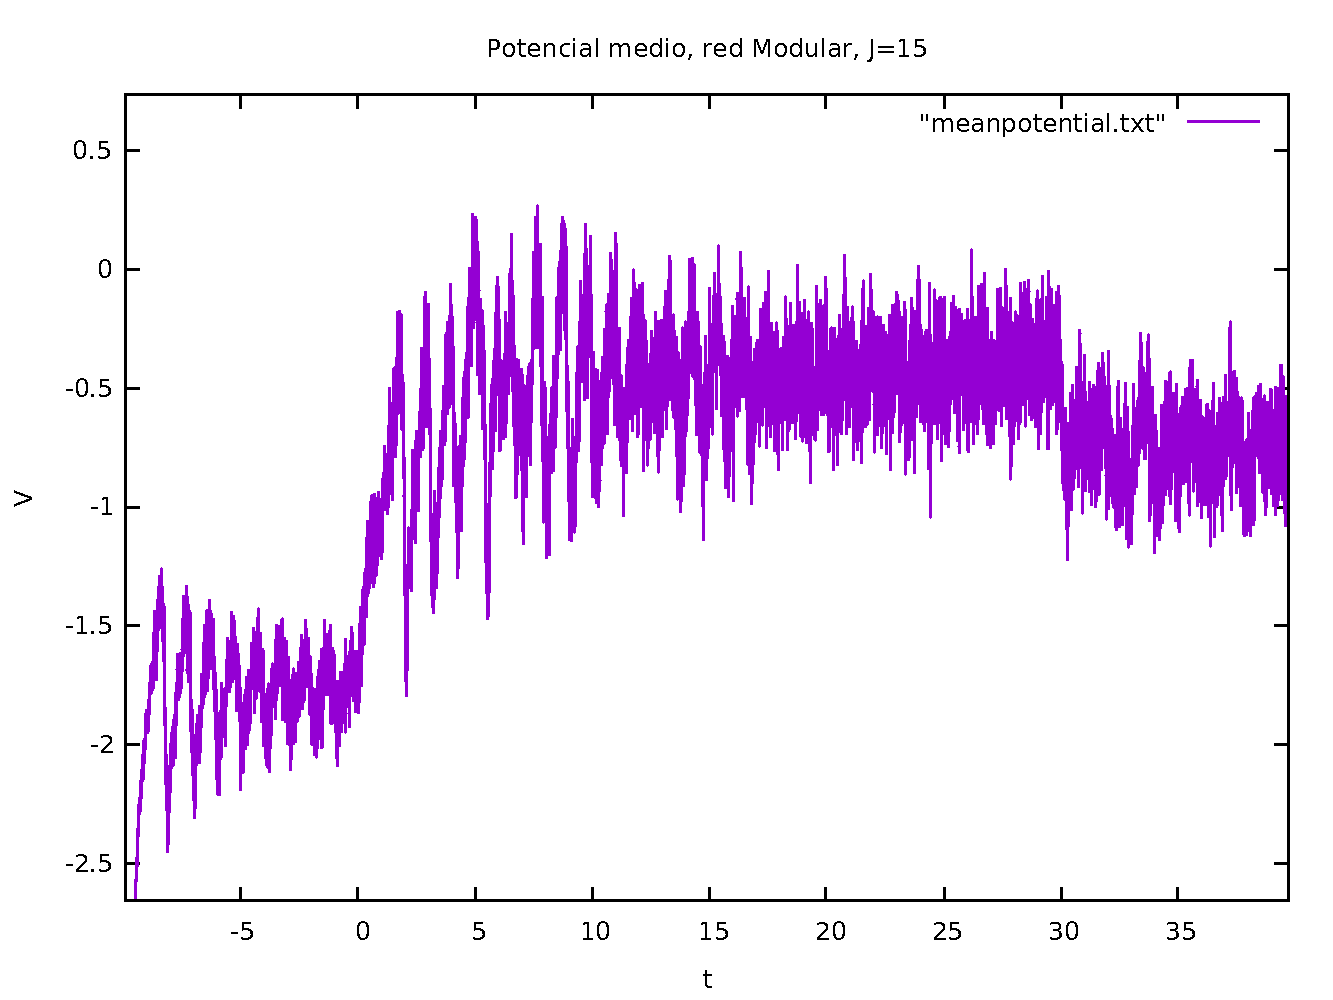
\includegraphics[scale=0.4]{modular_pot_J15.pdf}\\
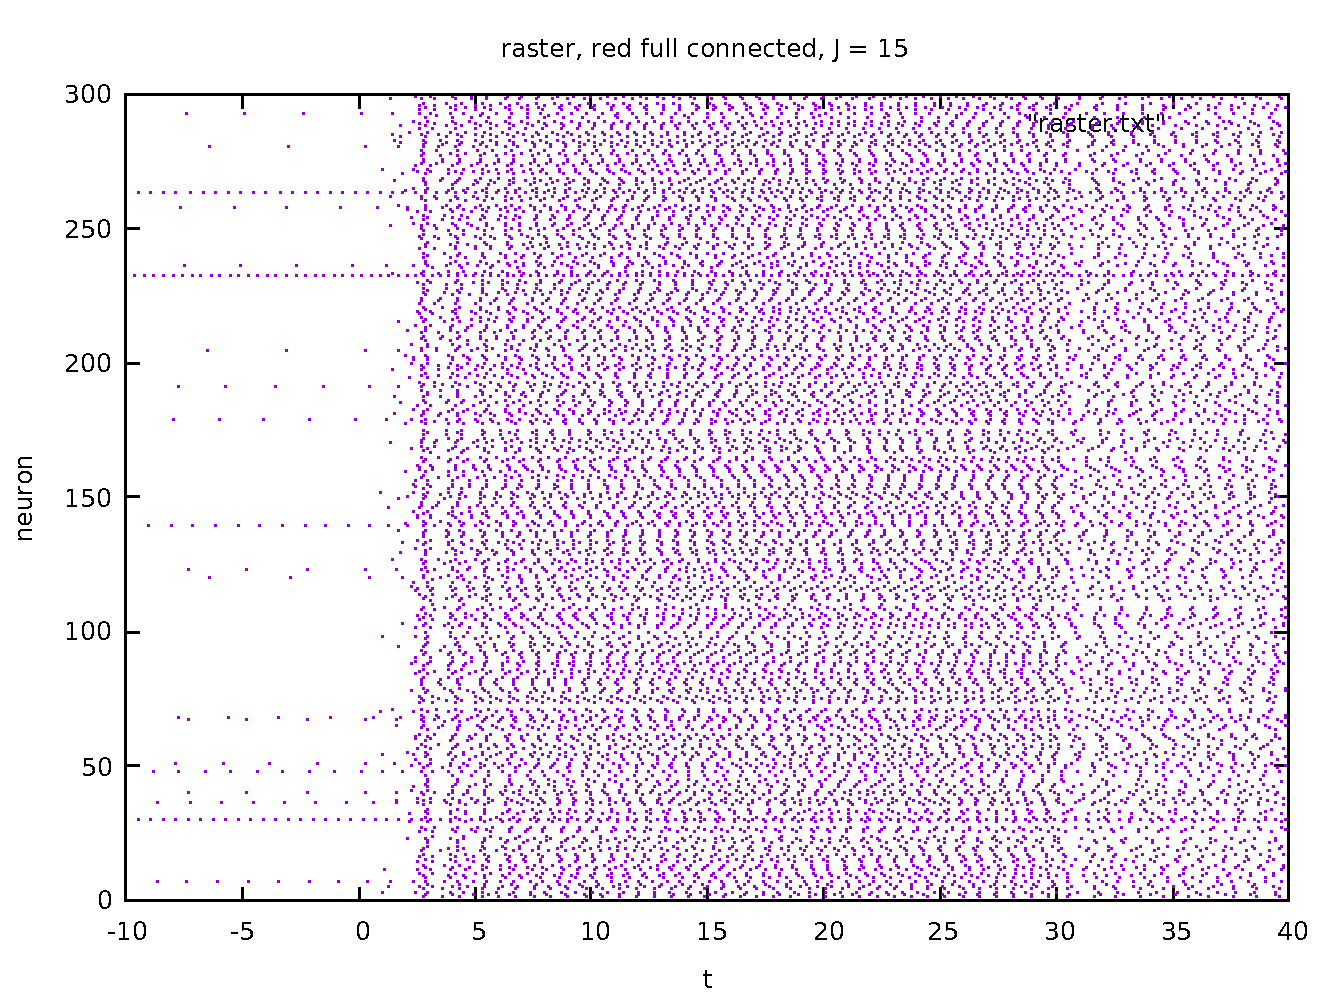
\includegraphics[width=10cm,height=5cm]{fullconnected_raster_J15.pdf}\\
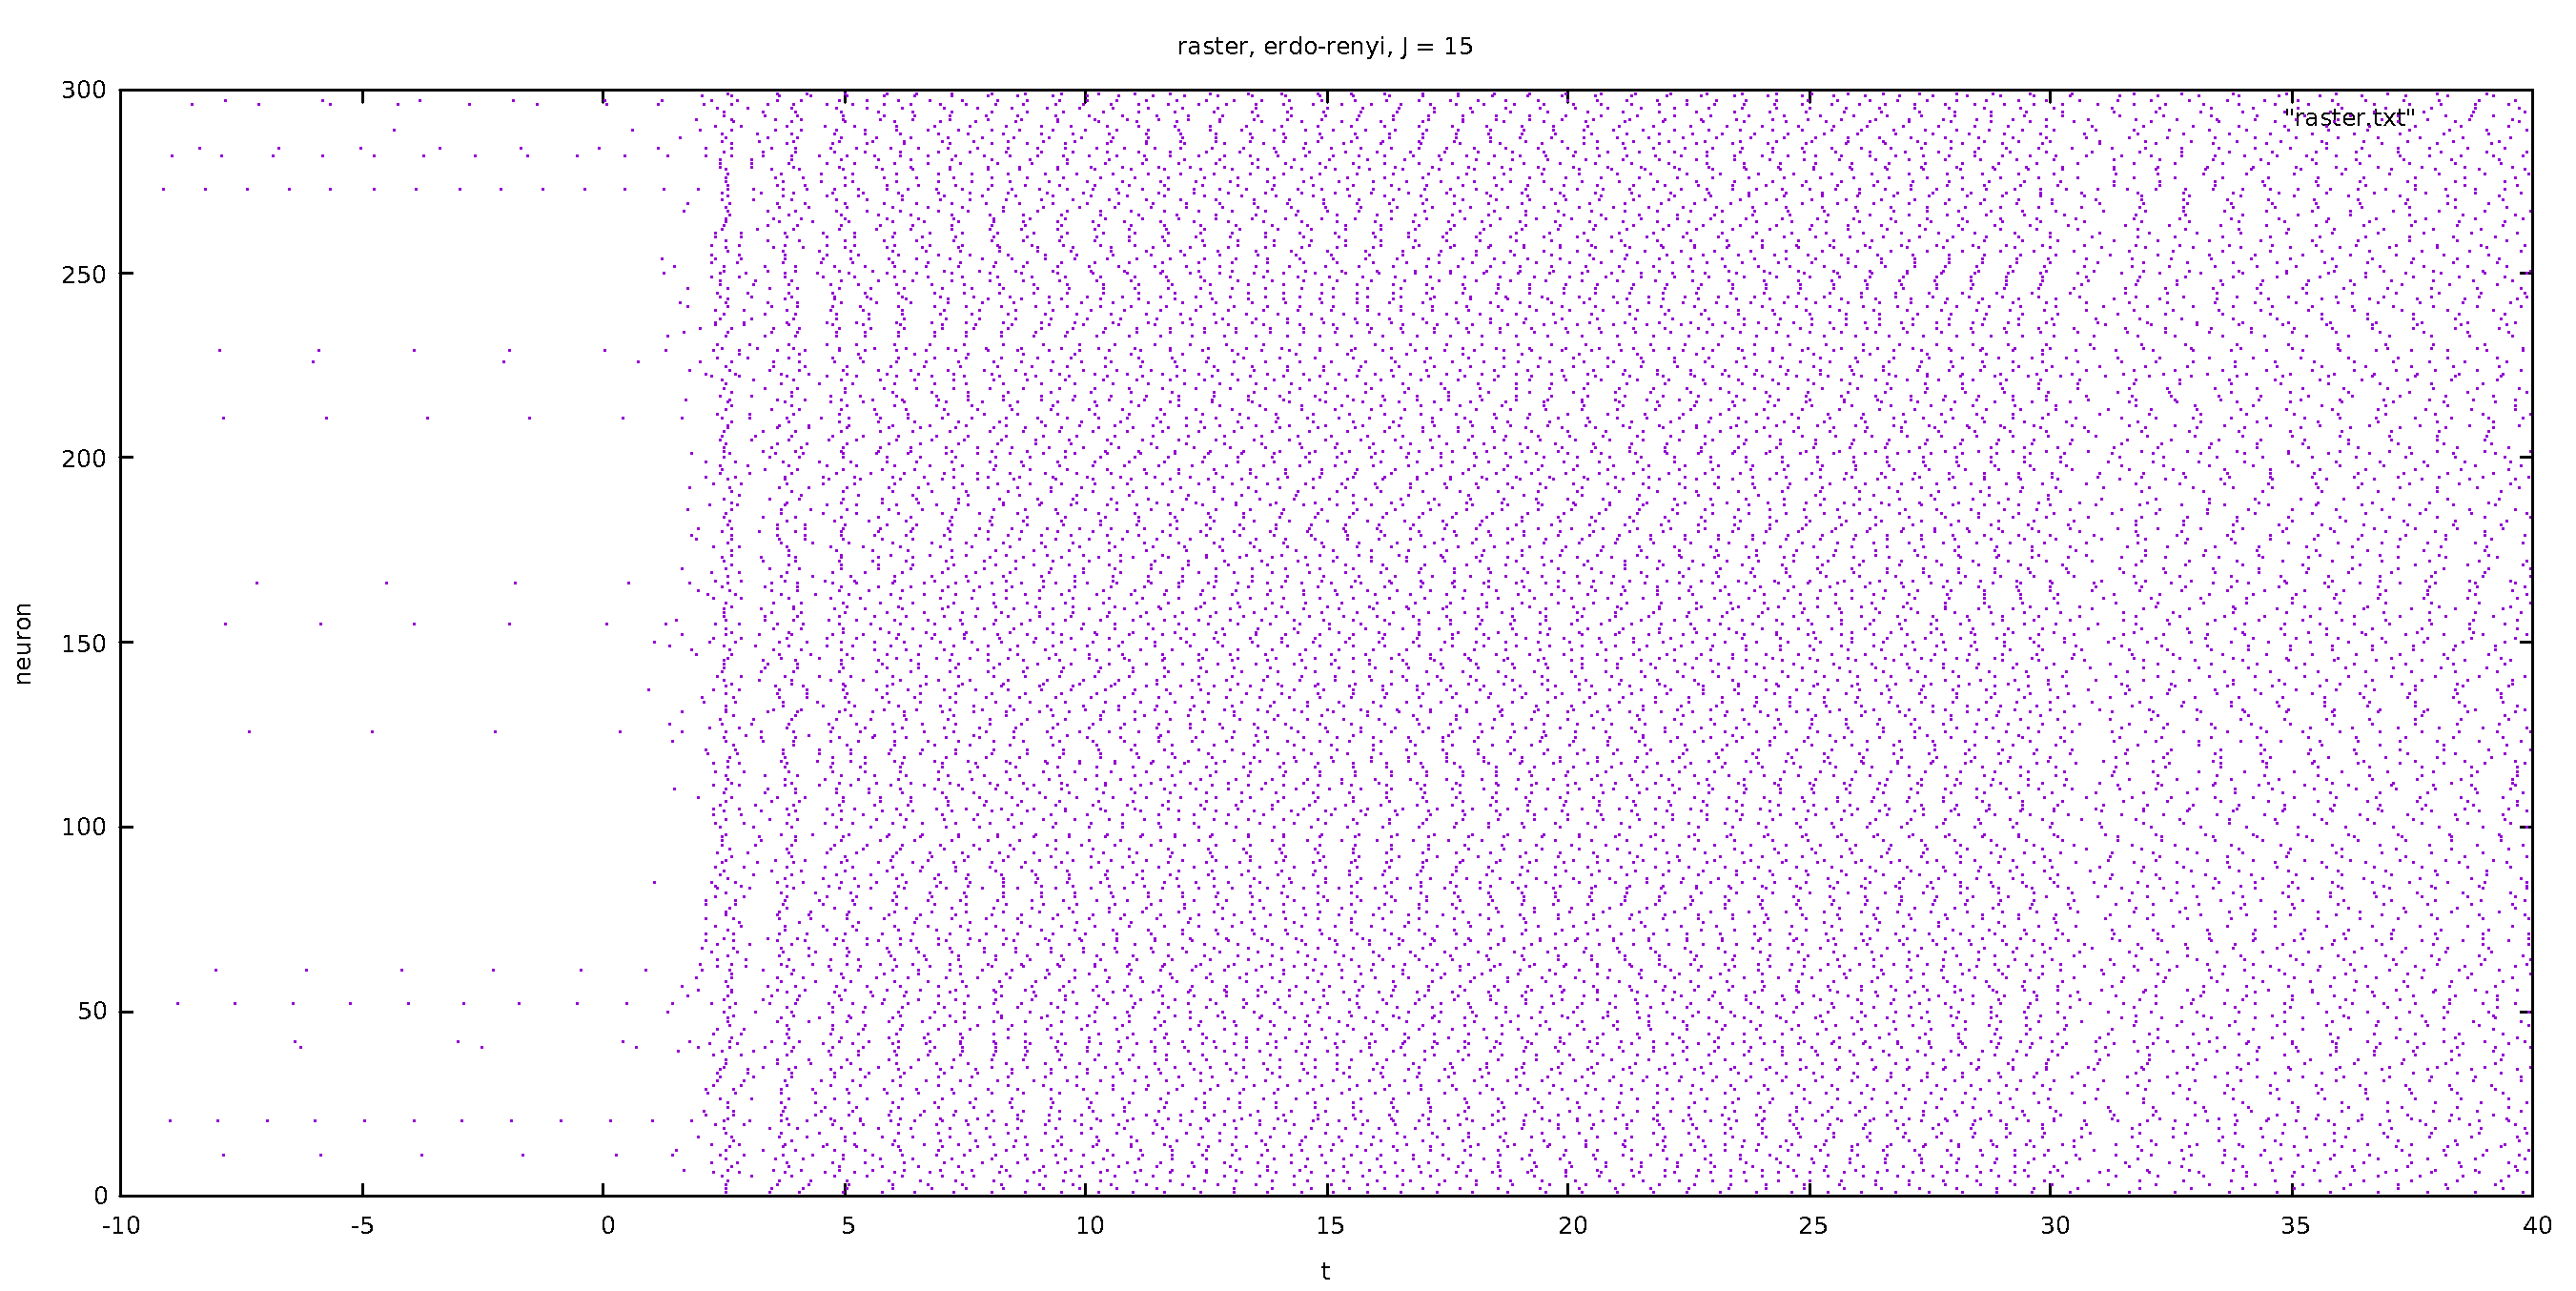
\includegraphics[width=10cm,height=5cm]{erdos_raster_J15.pdf}\\
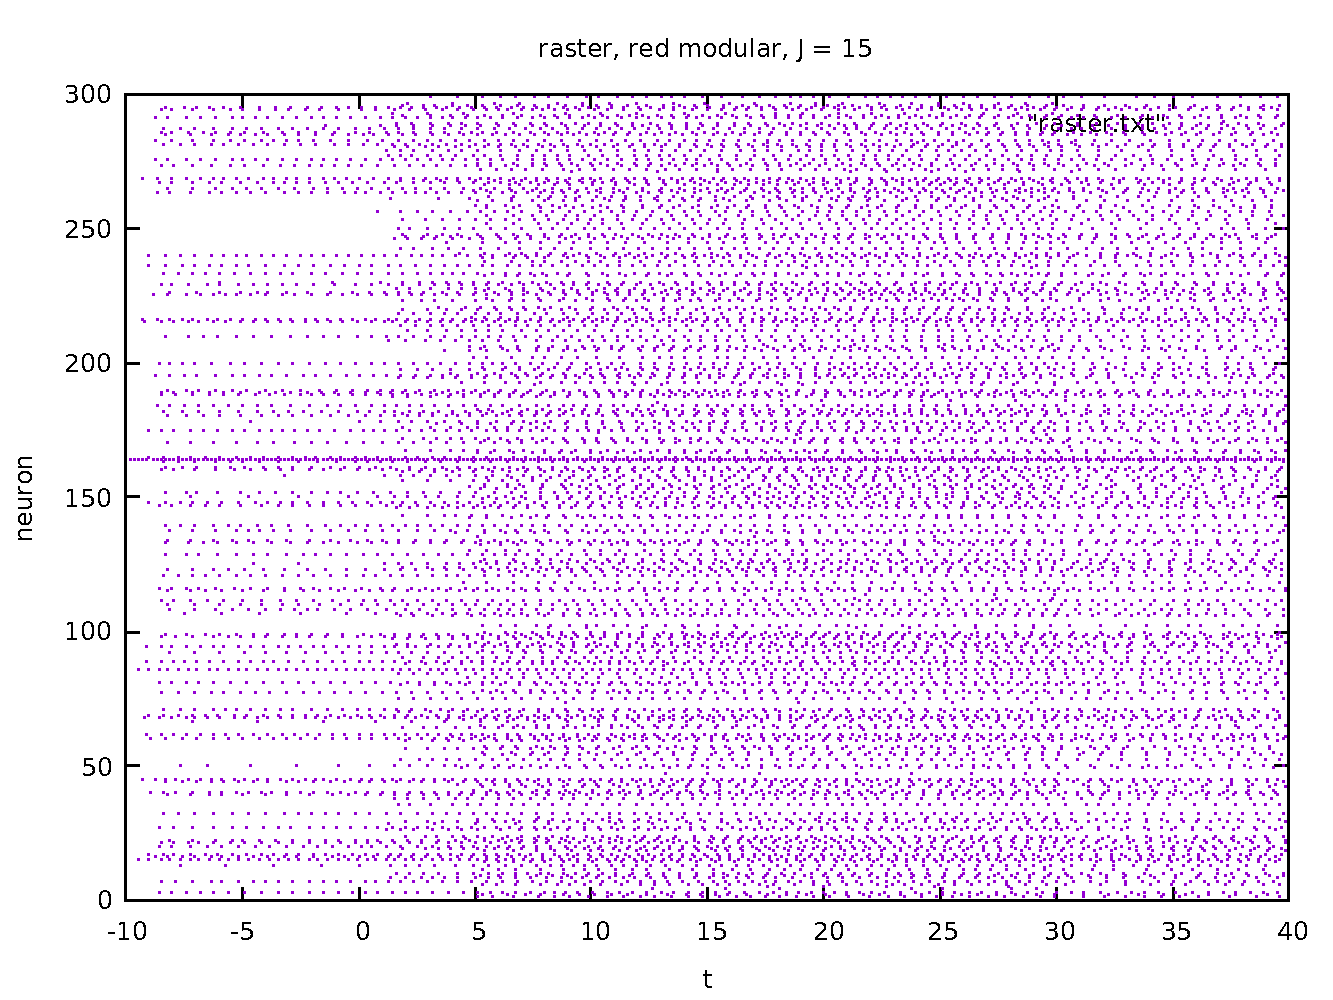
\includegraphics[width=10cm,height=5cm]{modular_raster_J15.pdf}\\
\subsection{raster semiordenado}
Si ordenamos el raster de forma que las primeras 100 neuronas corresponden al primer módulo, las 200 siguientes al segundo, etc, obtenemos un raster como el siguiente:\\
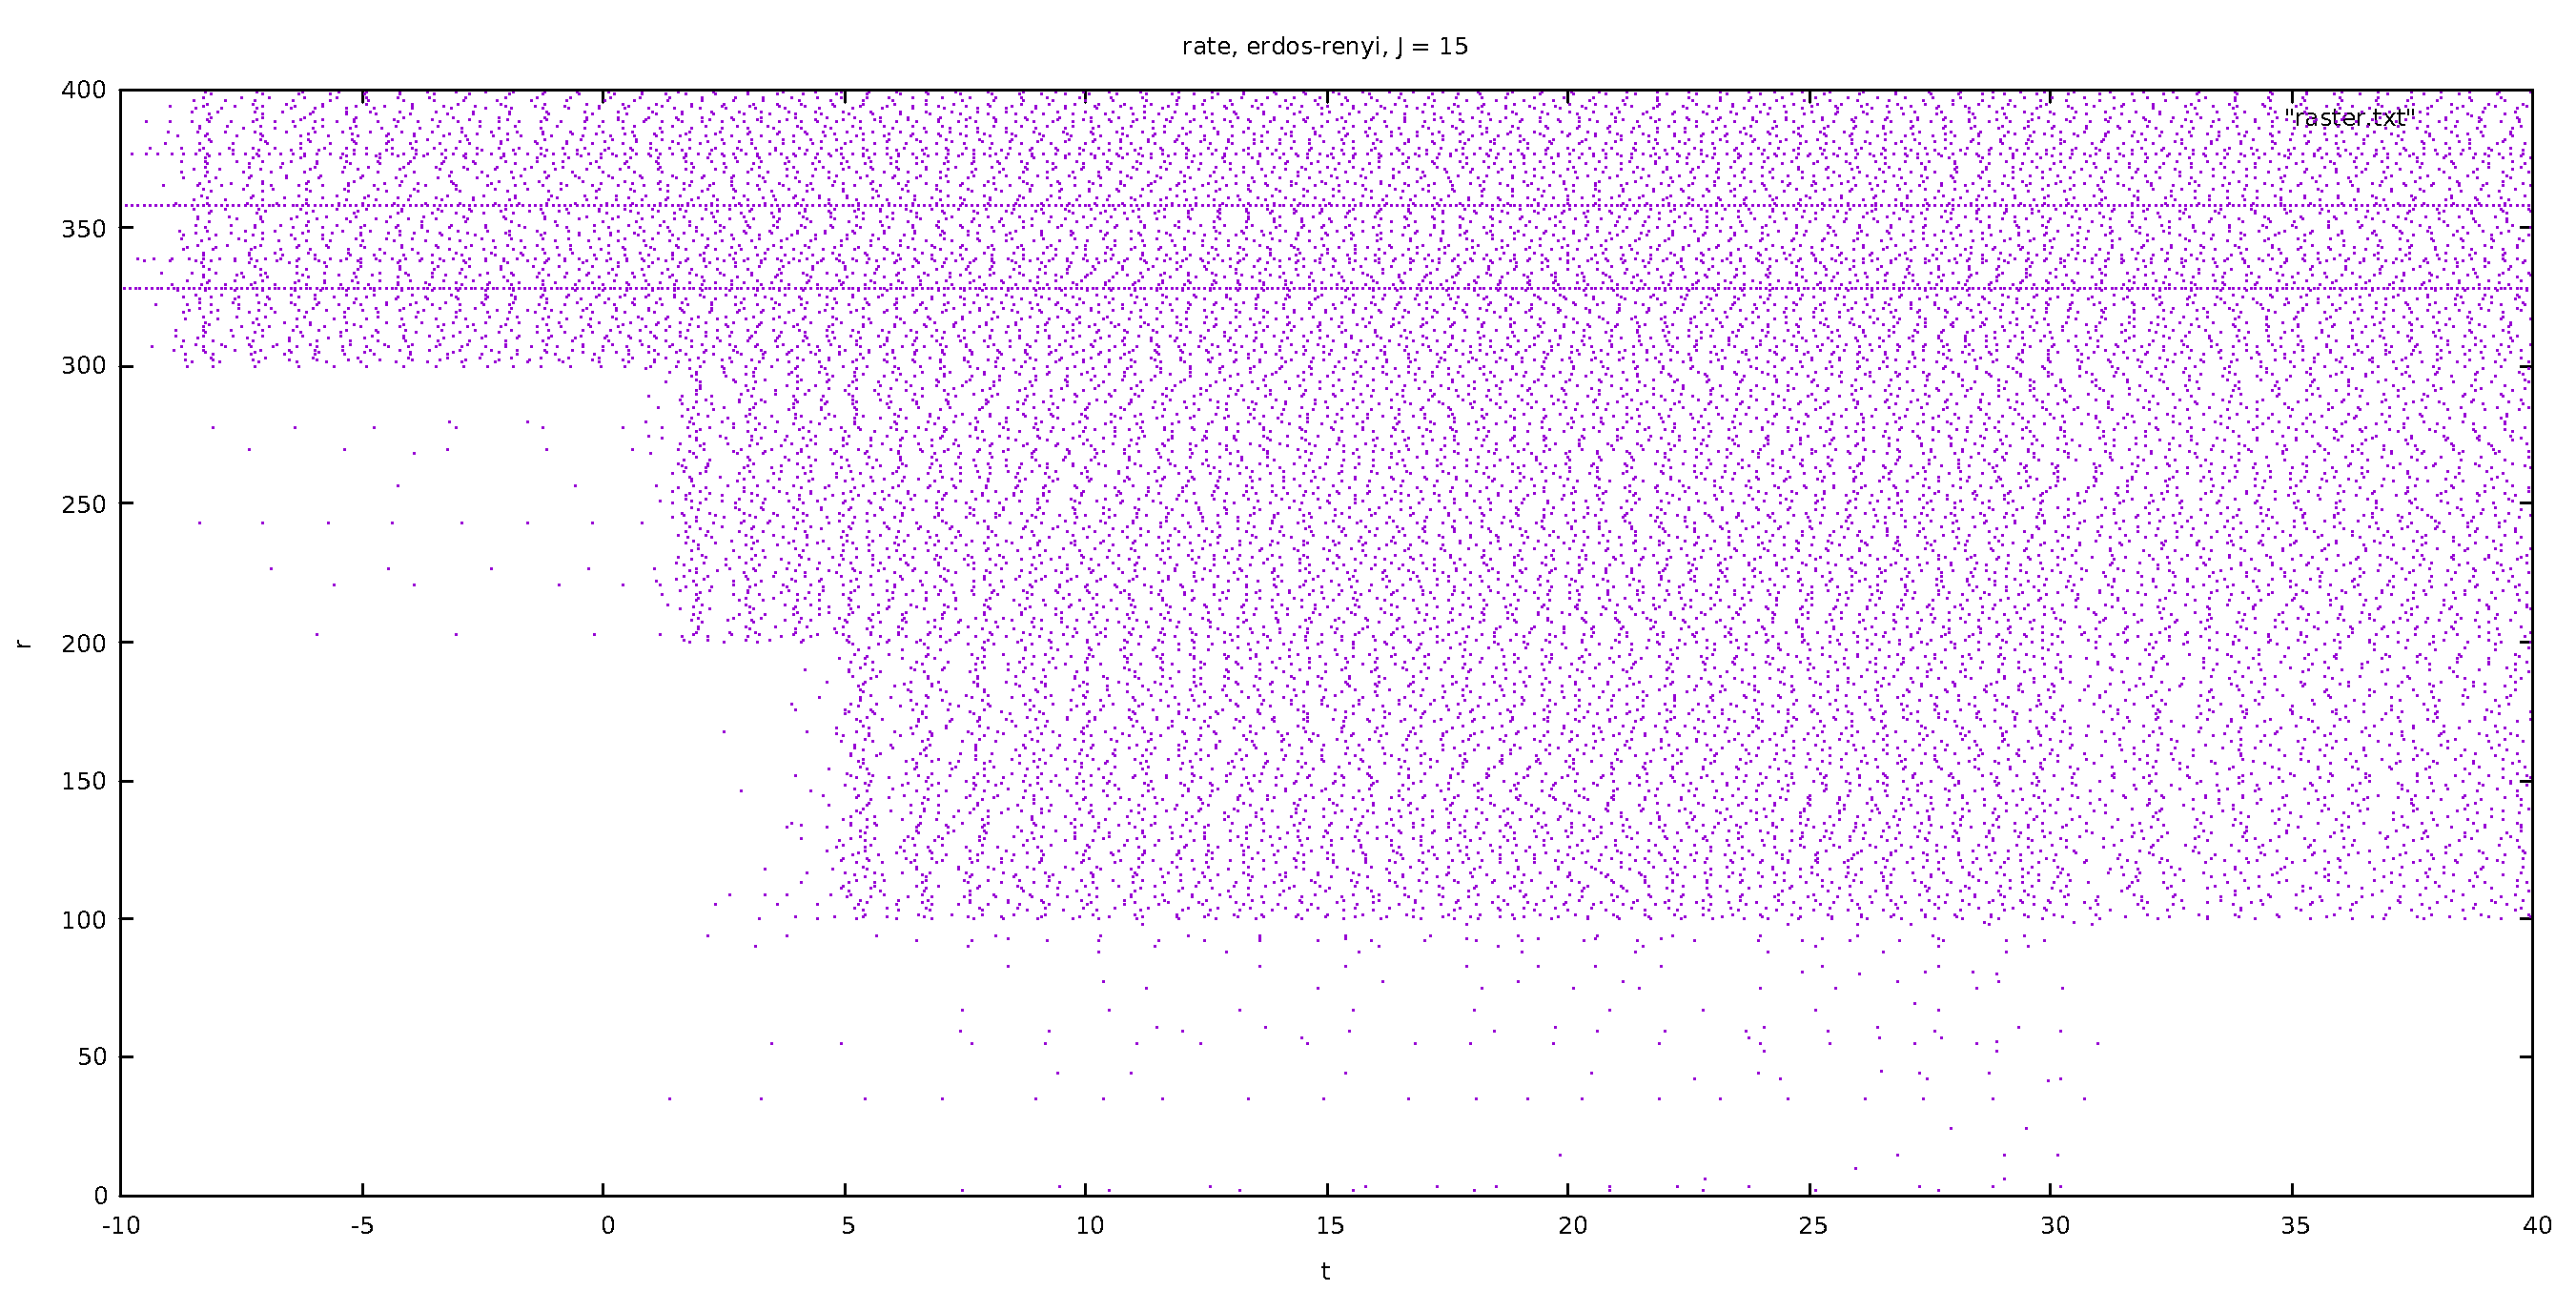
\includegraphics[width=10cm,height=5cm]{modular_raster_J15_semiorden.pdf}\\
donde vemos que cada bloque de neuronas se activa en momentos diferentes. Esto es así porque el valor de $\eta$ para cada neurona está ordenado. Por tanto, en el bloque 1 el valor de eta de las neuronas es mucho menor que su valor en el bloque 4. Si ordenamos las neuronas dentro de cada módulo nos queda la siguiente gráfica:\\
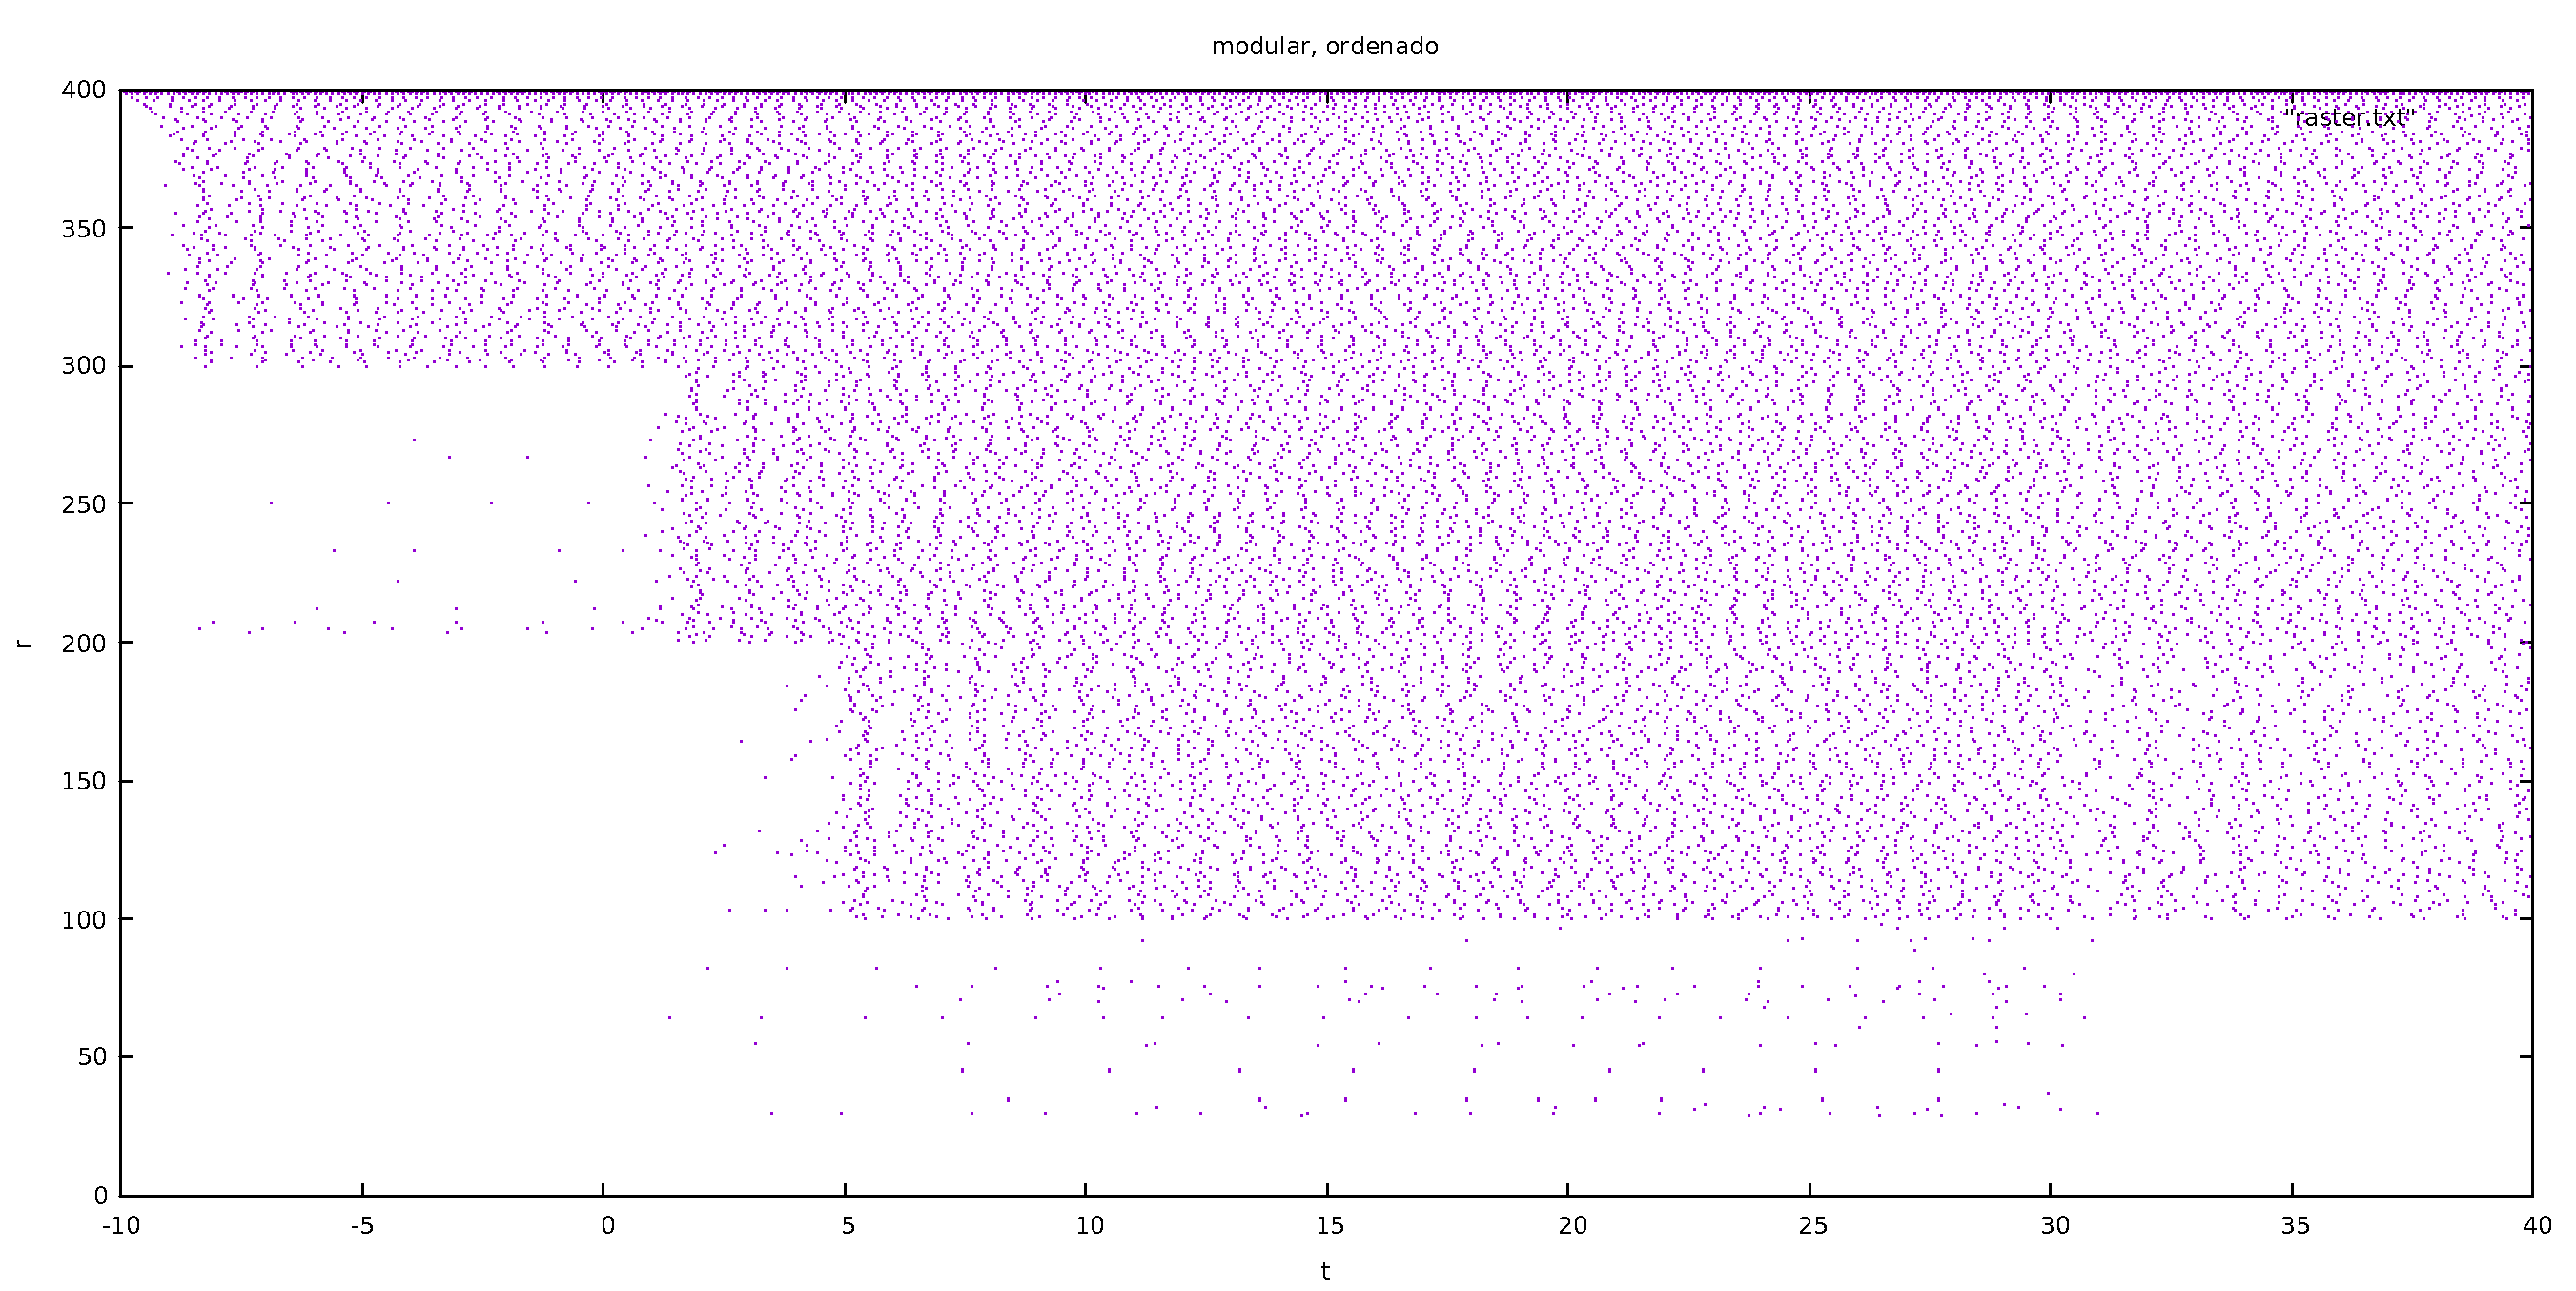
\includegraphics[width=10cm,height=5cm]{modular_raster_J15_orden.pdf}\\
Ahora solo introducimos corriente a uno de los módulos. Medimos el potencial medio, la tasa de disparo y las neuronas que se excitan para cada uno de los módulos:\\
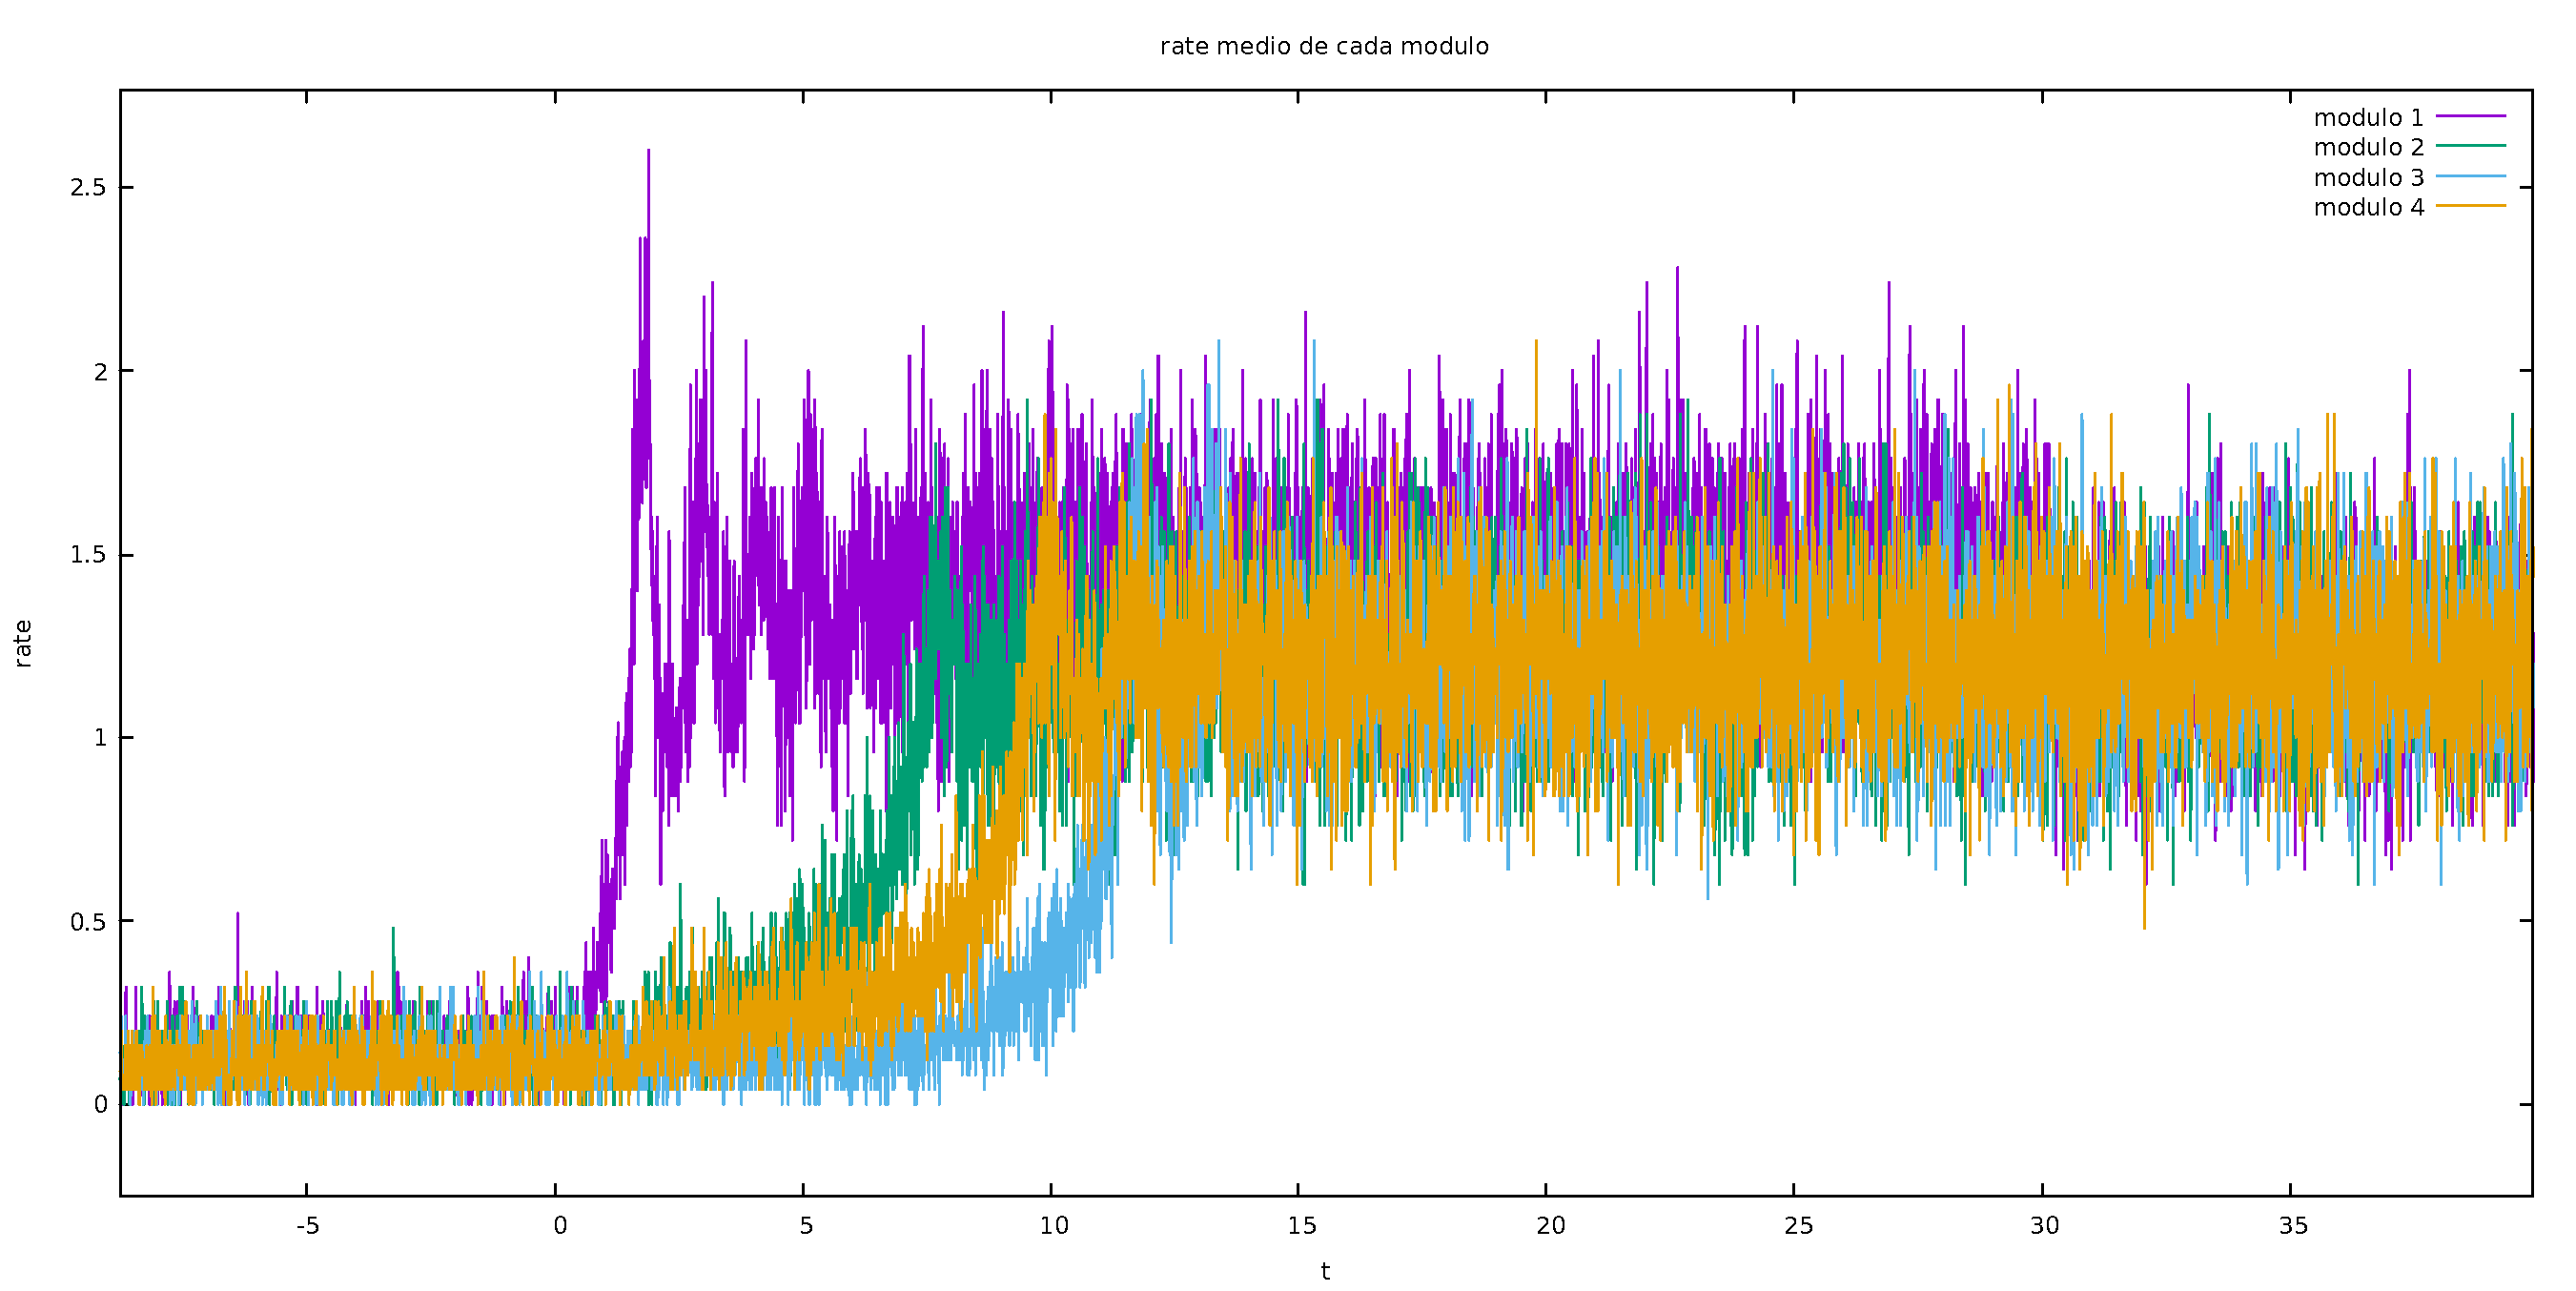
\includegraphics[width=10cm,height=5cm]{modular_rate_J15_separated.pdf}\\
\includegraphics[width=10cm,height=5cm]{modular_pot_J15_separated.pdf}\\
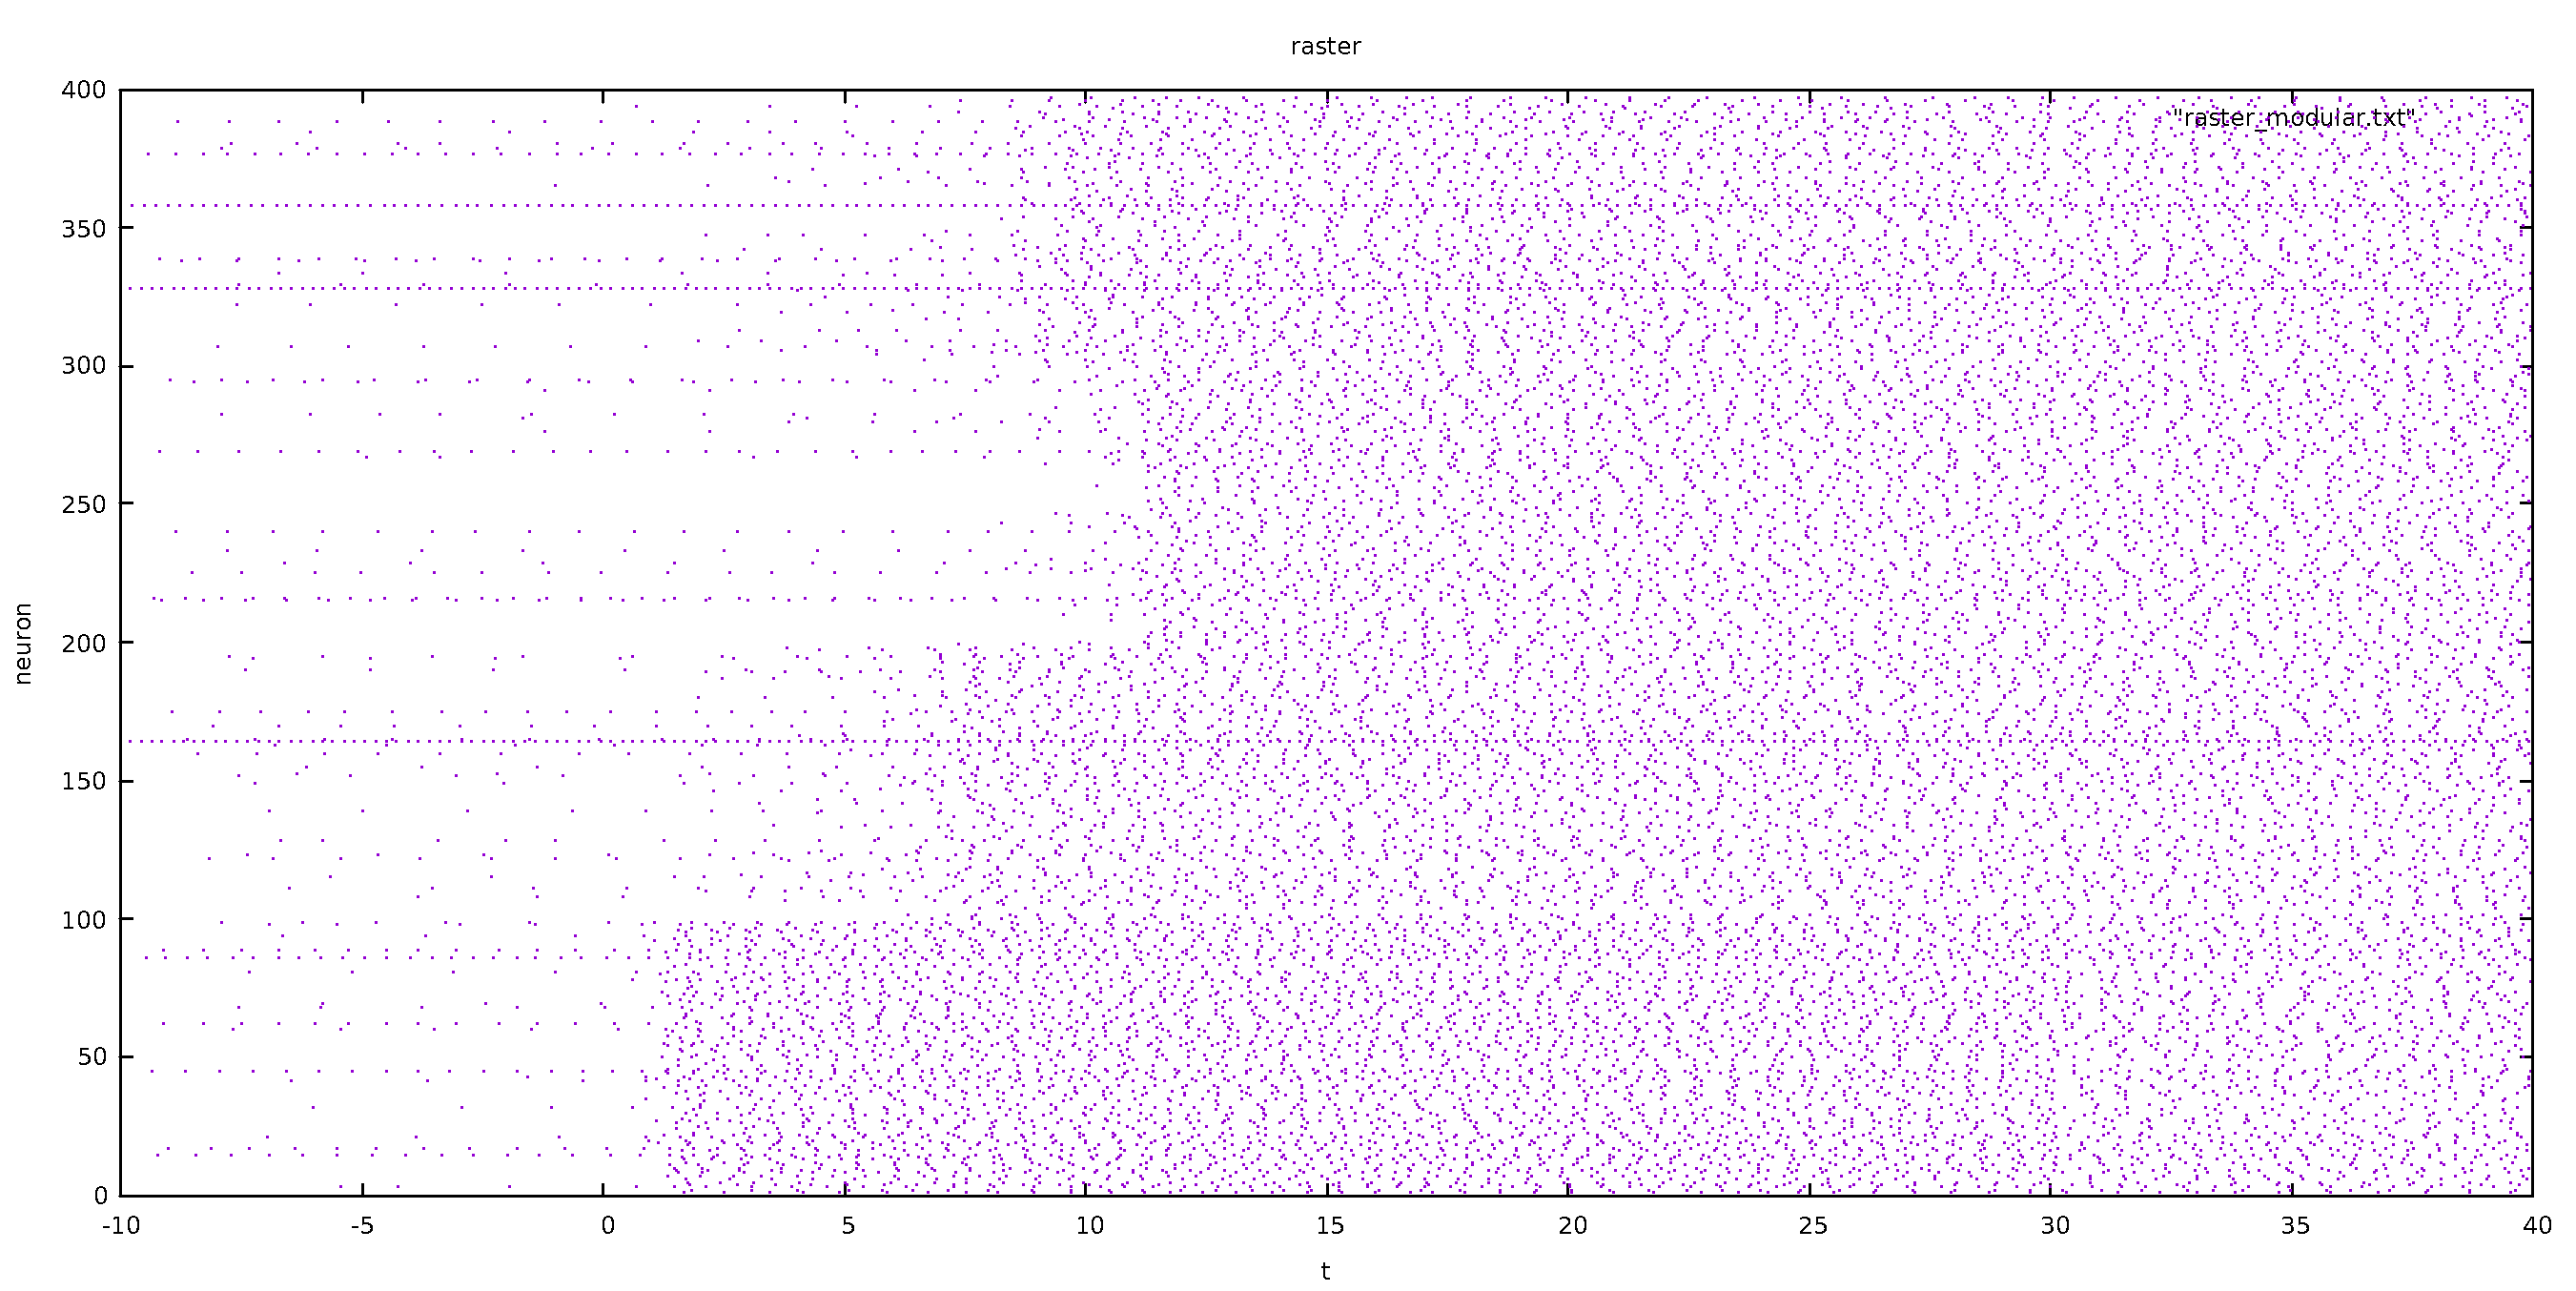
\includegraphics[width=10cm,height=5cm]{modular_raster_J15_separated.pdf}\\
Ahora aplicamos una corriente senoidal:\\
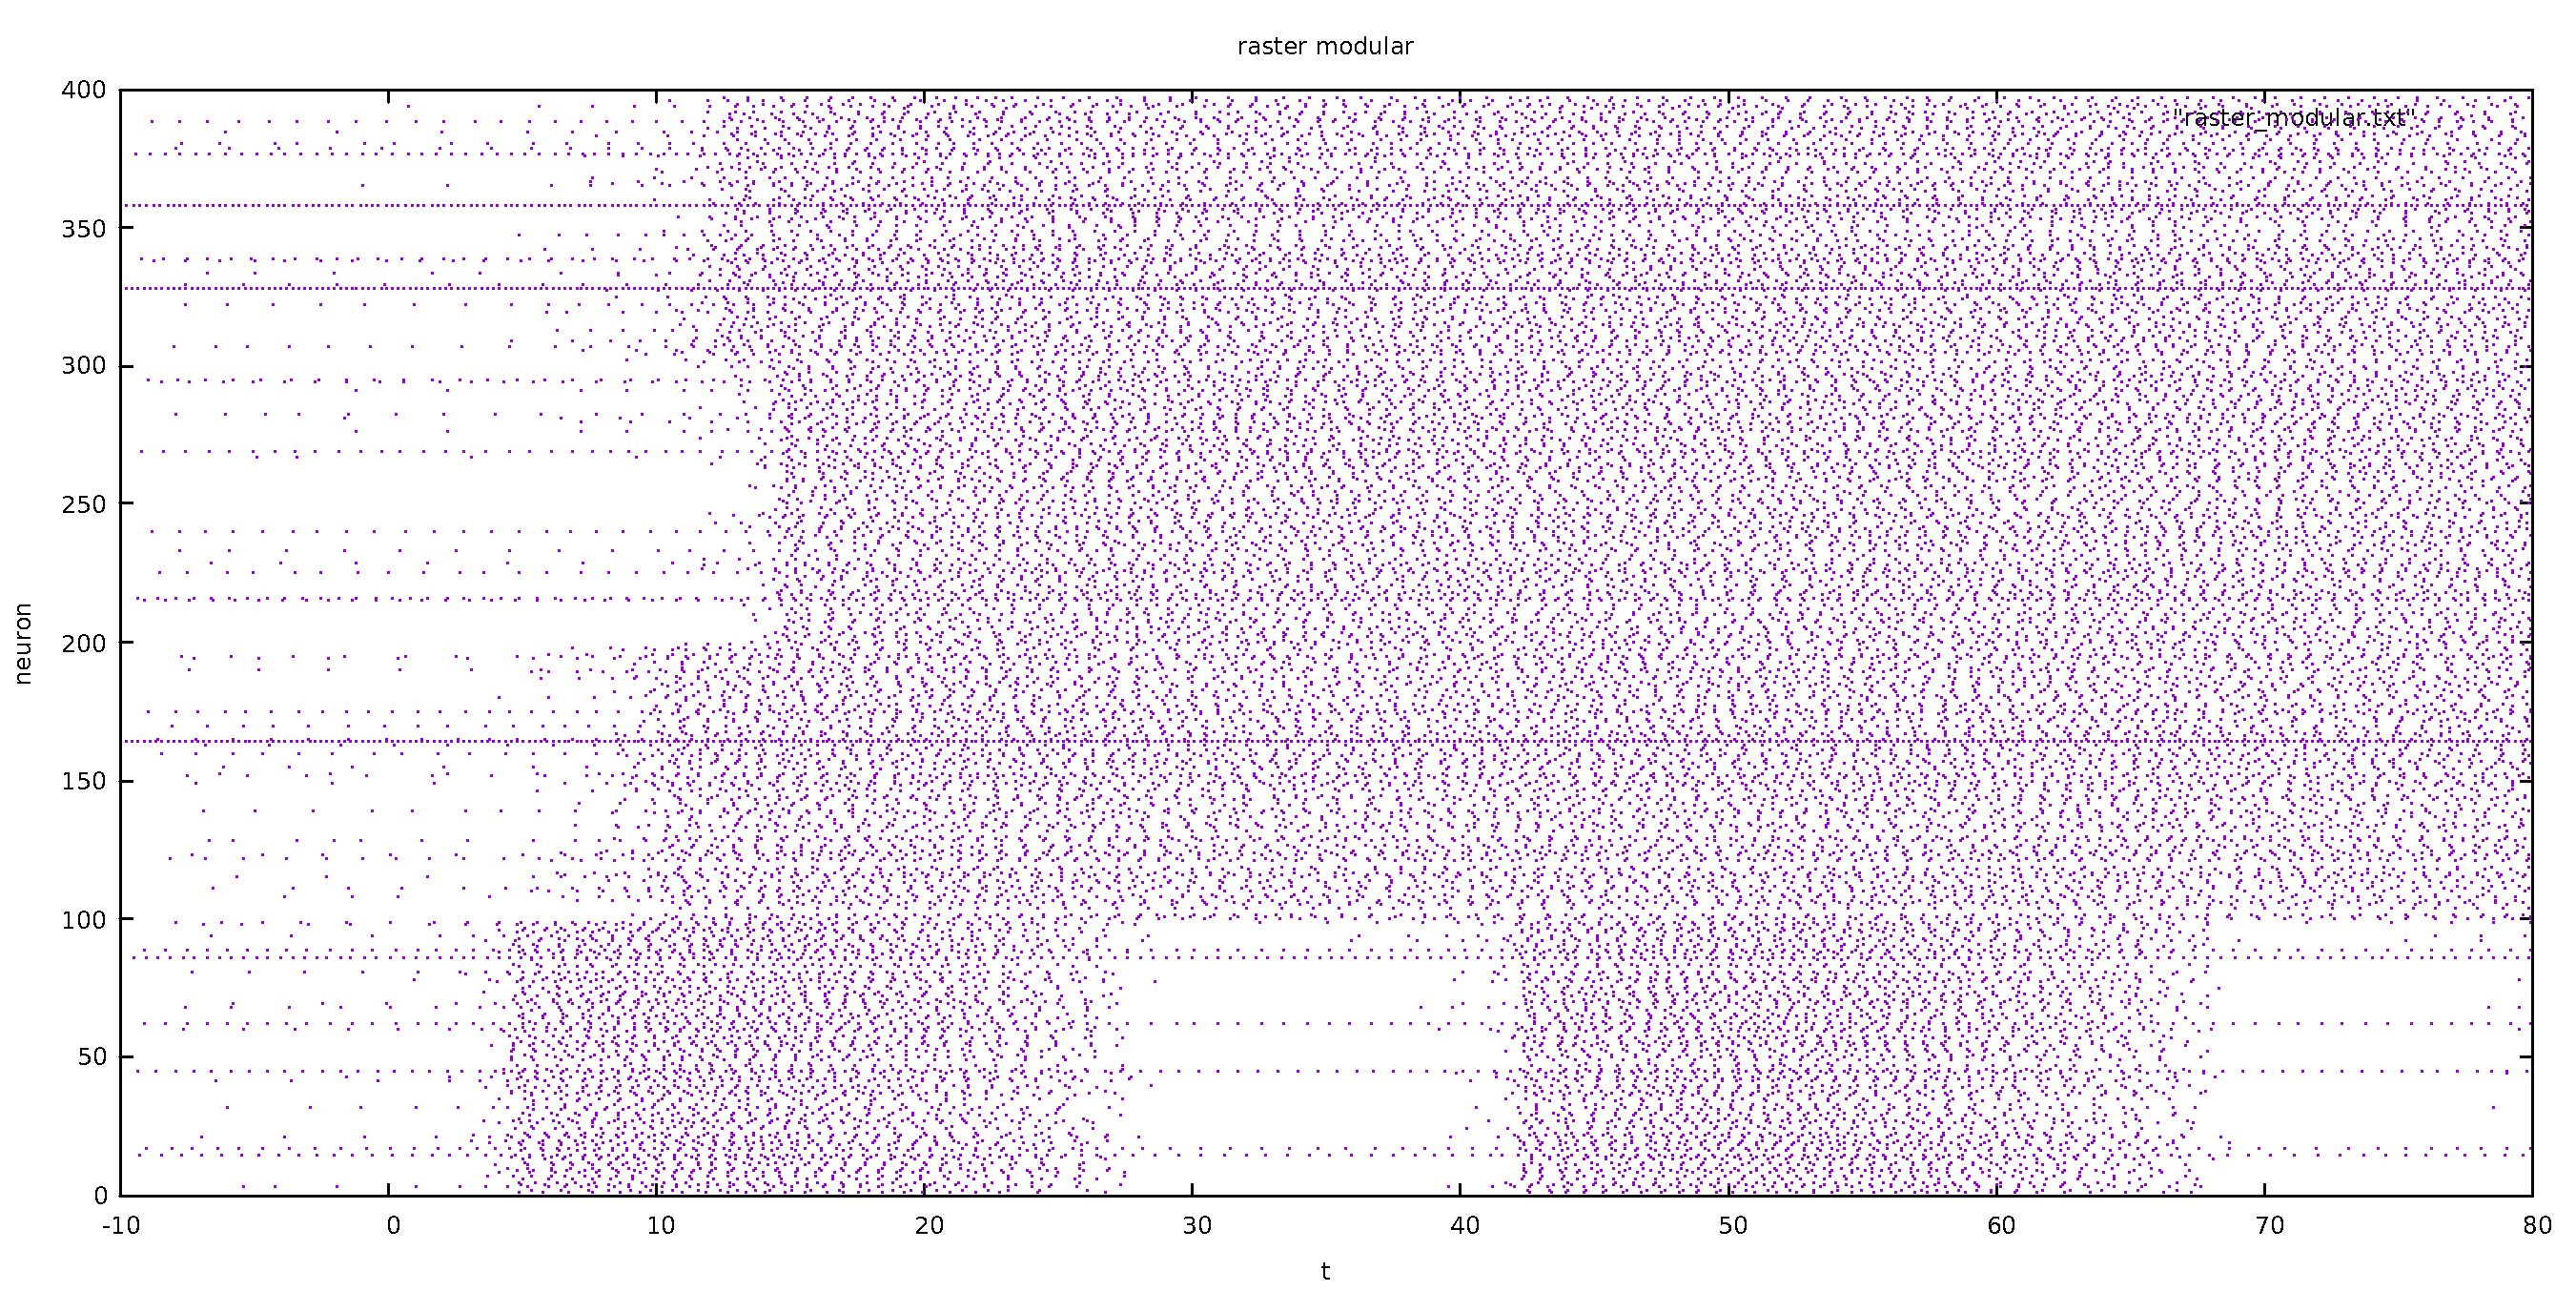
\includegraphics[width=10cm,height=5cm]{modular_raster_J15_separated_sin.pdf}\\
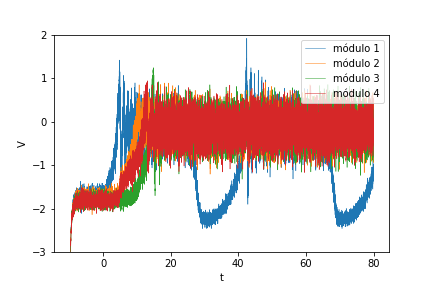
\includegraphics[width=10cm,height=5cm]{potencial_seno_modulos.png}\\
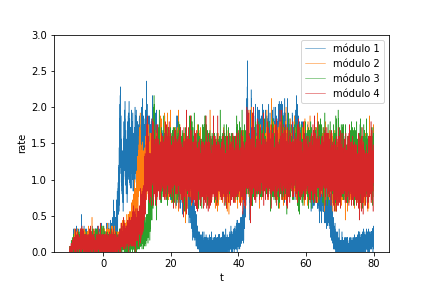
\includegraphics[width=10cm,height=5cm]{rate_seno_modulos.png}\\
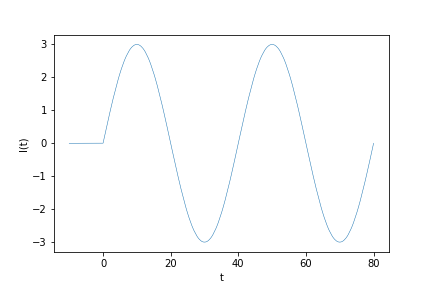
\includegraphics[width=10cm,height=5cm]{current_seno.png}\\
Para conectividad intramodular = 10 y conectividad intramodular = 1 tenemos la siguiente curva de estabilidad:\\
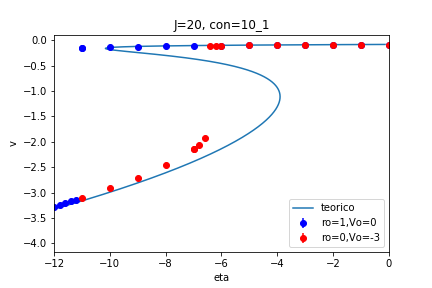
\includegraphics[scale=0.7]{v_vs_eta_J20_mod10_1.png}\\
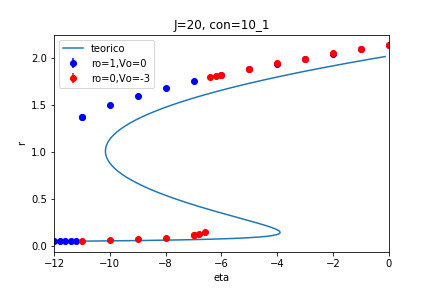
\includegraphics[scale=0.7]{r_vs_eta_J20_mod10_1.png}\\
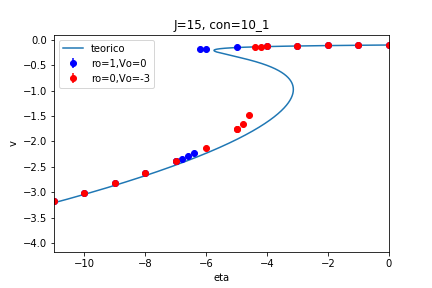
\includegraphics[scale=0.7]{v_vs_eta_J15_mod10_1.png}\\
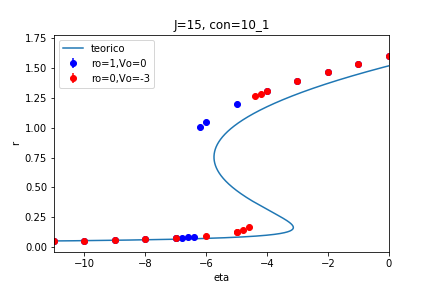
\includegraphics[scale=0.7]{r_vs_eta_J15_mod10_1.png}\\
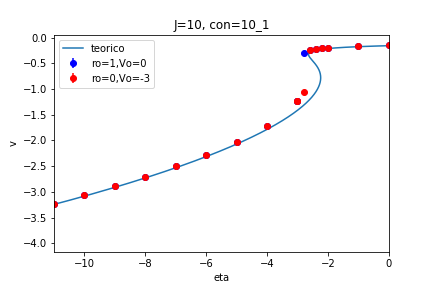
\includegraphics[scale=0.7]{v_vs_eta_J10_mod10_1.png}\\
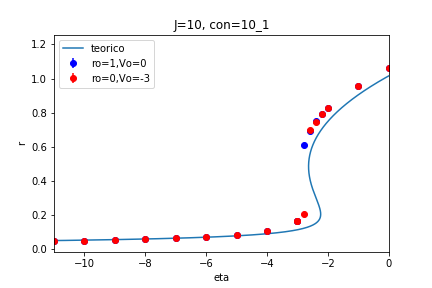
\includegraphics[scale=0.7]{r_vs_eta_J10_mod10_1.png}\\
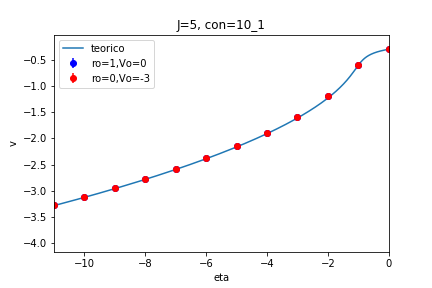
\includegraphics[scale=0.7]{v_vs_eta_J5_mod10_1.png}\\
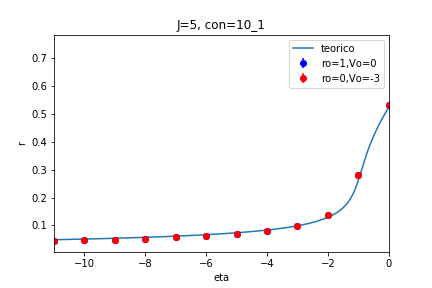
\includegraphics[scale=0.7]{r_vs_eta_J5_mod10_1.png}\\
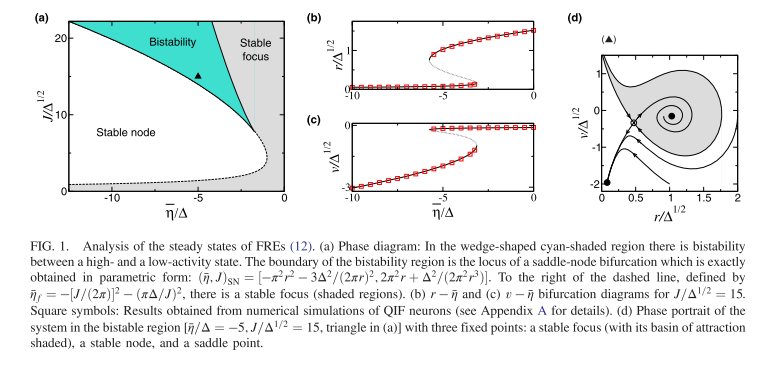
\includegraphics[scale=0.4]{diagramaspaper.png}\\
Para conectividad intramodular = 10 y conectividad intramodular = 1 tenemos la siguiente curva de estabilidad:\\
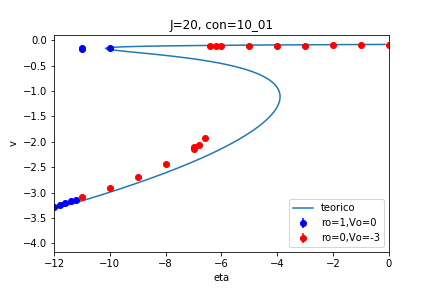
\includegraphics[scale=0.7]{v_vs_eta_J20_mod10_01.png}\\
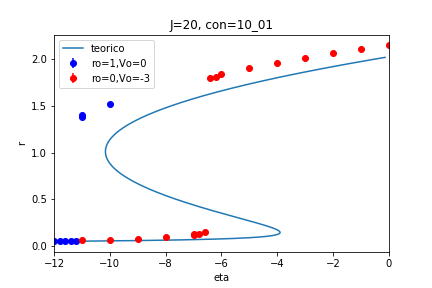
\includegraphics[scale=0.7]{r_vs_eta_J20_mod10_01.png}\\
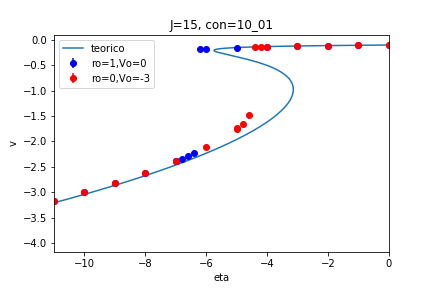
\includegraphics[scale=0.7]{v_vs_eta_J15_mod10_01.png}\\
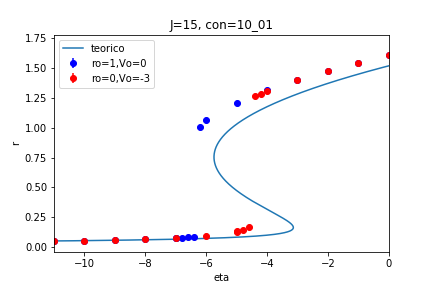
\includegraphics[scale=0.7]{r_vs_eta_J15_mod10_01.png}\\
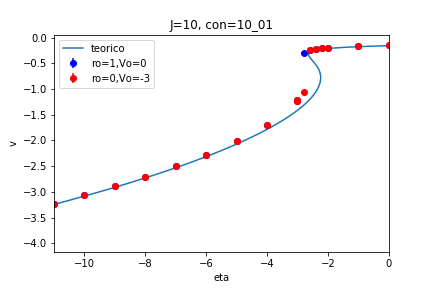
\includegraphics[scale=0.7]{v_vs_eta_J10_mod10_01.png}\\
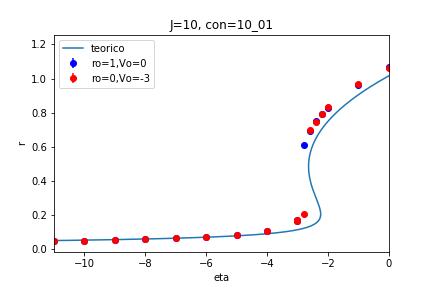
\includegraphics[scale=0.7]{r_vs_eta_J10_mod10_01.png}\\
\includegraphics[scale=0.7]{v_vs_eta_J5_mod10_01.png}\\
\includegraphics[scale=0.7]{r_vs_eta_J5_mod10_01.png}\\


\end{document}
